\documentclass[12pt]{article}
\usepackage[utf8]{inputenc}
\usepackage[english]{babel}
\usepackage[a4paper, total={7.25in, 9.5in}]{geometry}
\usepackage{tikz-feynman}
\tikzfeynmanset{compat=1.0.0} 
\usepackage{subcaption}
\usepackage{float}
\floatplacement{figure}{H}
\usepackage{simplewick}
 
\newcommand{\field}{\hat{\Phi}}
\newcommand{\dfield}{\hat{\Phi}^\dagger}
 
\usepackage{amsthm, amssymb, amsmath, centernot}
\usepackage{slashed}
\newcommand{\notimplies}{%
  \mathrel{{\ooalign{\hidewidth$\not\phantom{=}$\hidewidth\cr$\implies$}}}}
 
\renewcommand\qedsymbol{$\square$}
\newcommand{\cont}{$\boxtimes$}
\newcommand{\divides}{\mid}
\newcommand{\ndivides}{\centernot \mid}
\newcommand{\Z}{\mathbb{Z}}
\newcommand{\N}{\mathbb{N}}
\newcommand{\C}{\mathbb{C}}
\newcommand{\Zplus}{\mathbb{Z}^{+}}
\newcommand{\Primes}{\mathbb{P}}
\newcommand{\ball}[2]{B_{#1} \! \left(#2 \right)}
\newcommand{\Q}{\mathbb{Q}}
\newcommand{\R}{\mathbb{R}}
\newcommand{\Rplus}{\mathbb{R}^+}
\newcommand{\invI}[2]{#1^{-1} \left( #2 \right)}
\newcommand{\End}[1]{\text{End}\left( A \right)}
\newcommand{\legsym}[2]{\left(\frac{#1}{#2} \right)}
\renewcommand{\mod}[3]{\: #1 \equiv #2 \: \mathrm{mod} \: #3 \:}
\newcommand{\nmod}[3]{\: #1 \centernot \equiv #2 \: mod \: #3 \:}
\newcommand{\ndiv}{\hspace{-4pt}\not \divides \hspace{2pt}}
\newcommand{\finfield}[1]{\mathbb{F}_{#1}}
\newcommand{\finunits}[1]{\mathbb{F}_{#1}^{\times}}
\newcommand{\ord}[1]{\mathrm{ord}\! \left(#1 \right)}
\newcommand{\quadfield}[1]{\Q \small(\sqrt{#1} \small)}
\newcommand{\vspan}[1]{\mathrm{span}\! \left\{#1 \right\}}
\newcommand{\galgroup}[1]{Gal \small(#1 \small)}
\newcommand{\bra}[1]{\left| #1 \right>}
\newcommand{\Oa}{O_\alpha}
\newcommand{\Od}{O_\alpha^{\dagger}}
\newcommand{\Oap}{O_{\alpha '}}
\newcommand{\Odp}{O_{\alpha '}^{\dagger}}
\renewcommand{\Im}[1]{\mathrm{Im} \: #1}
\newcommand{\ket}[1]{\left| #1 \right>}
\renewcommand{\bra}[1]{\left< #1 \right|}
\newcommand{\inner}[2]{\left< #1 | #2 \right>}
\newcommand{\expect}[2]{\left< #1 \right| #2 \left| #1 \right>}
\renewcommand{\d}[1]{ \mathrm{d}#1 \:}
\newcommand{\dn}[2]{ \mathrm{d}^{#1} #2 \:}
\newcommand{\deriv}[2]{\frac{\d{#1}}{\d{#2}}}
\newcommand{\pderiv}[2]{\frac{\partial{#1}}{\partial{#2}}}
\newcommand{\parsq}[2]{\frac{\partial^2{#1}}{\partial{#2}^2}}
\newcommand{\topo}{\mathcal{T}}
\newcommand{\base}{\mathcal{B}}
\renewcommand{\bf}[1]{\mathbf{#1}}
\renewcommand{\a}{\hat{a}}
\newcommand{\adag}{\hat{a}^\dagger}
\renewcommand{\b}{\hat{b}}
\newcommand{\bdag}{\hat{b}^\dagger}
\newcommand{\cdag}{\hat{c}^\dagger}
\newcommand{\hamilt}{\hat{H}}
\renewcommand{\L}{\hat{L}}
\newcommand{\Lz}{\hat{L}_z}
\newcommand{\Lsquared}{\hat{L}^2}
\renewcommand{\S}{\hat{S}}
\renewcommand{\empty}{\varnothing}
\newcommand{\J}{\hat{J}}
\newcommand{\lagrange}{\mathcal{L}}
\newcommand{\dfourx}{\mathrm{d}^4x}
\newcommand{\meson}{\phi}
\newcommand{\dpsi}{\psi^\dagger}
\newcommand{\ipic}{\mathrm{int}}
\newcommand{\parity}{\mathbf{P}}
\newcommand{\conj}{\mathbf{C}}
\newcommand{\tr}[1]{\mathrm{Tr} \left( #1 \right)}

\renewcommand{\theenumi}{(\alph{enumi})}

\newcommand{\atitle}[1]{\title{% 
	\large \textbf{Physics GR6047 Quantum Field Theory I
	\\ Assignment \# #1} \vspace{-2ex}}
\author{Benjamin Church }
\maketitle}

 
\newtheorem{theorem}{Theorem}[section]
\newtheorem{lemma}[theorem]{Lemma}
\newtheorem{proposition}[theorem]{Proposition}
\newtheorem{corollary}[theorem]{Corollary}
\newtheorem{remark}[theorem]{Remark}
 



\begin{document}
\newcommand{\MeV}{\: \mathrm{MeV}}
\newcommand{\GeV}{\: \mathrm{GeV}}

\title{% 
	\large \textbf{Physics GR6047 Quantum Field Theory I
	\\ Final Exam \vspace{-2ex}}
\author{Benjamin Church }
}
\maketitle

\section{}

\newcommand{\cmat}{\mathcal{C}}
\newcommand{\gs}{g_e}
\newcommand{\gp}{g_o}

Consider the QED Lagrangian,
\[ \lagrange_{QED} = - \tfrac{1}{4} F_{\mu \nu} F^{\mu \nu} + \bar{\psi} (i \gamma^\mu \mathcal{D}_\mu - m ) \psi \]
We can express charge conjugation as its matrix action via,
\[\conj^{-1} \psi(x) \conj = \mathcal{C} \cdot \psi(x)^* \]
where $\mathcal{C} = i \gamma^2$. 
In the chiral basis,
\[ (\gamma^\mu)^* = \gamma^2 \gamma^\mu \gamma^2 = - \mathcal{C} \gamma^\mu  \mathcal{C} \]
This can be checked directly or by noting that $\gamma^2$ is the only complex gamma matrix in the chiral basis,
\[ \gamma^2 \gamma^\mu \gamma^2 = - \gamma^\mu (\gamma^2)^2 + 2 \eta^{\mu 2}  \gamma^2 = \gamma^\mu + 2 \eta^{\mu 2}  \gamma^2 = (\gamma^\mu)^* \]
I need a few more facts,
\[ \conj^{-1} \bar{\psi}(x) \conj = (\conj^{-1} \psi(x) \conj)^{\dagger} \gamma^0 = \left(\mathcal{C} \cdot \psi^*(x) \right)^\dagger \gamma^0 = \psi^{\top}(x) \mathcal{C}^\dagger \gamma^0 = - \psi^{\top}(x) i \gamma^0 \gamma^2 (\gamma^0)^2 = - \bar{\psi}^* i \gamma^2 = - \bar{\psi}^{*} \cdot \mathcal{C} \]    
and $\mathcal{C} = i \gamma^2$ is Hermitian because,
\[ \mathcal{C}^\dagger = (i \gamma^2)^\dagger = -i \gamma^0 \gamma^2 \gamma^0 = i(\gamma^0)^2 \gamma^2 = i \gamma^2 = \mathcal{C} \]
Now I have enough information to attack the Lagrangian. I propose the transformation,
\[ \conj^{-1} A_\mu(x) \conj = - A_\mu(x) \quad \text{and thus} \quad \conj^{-1} F_{\mu \nu} \conj = F_{\mu \nu}\]
since charge conjugation ought to change the sign of the electric charge. This indeed works. We will consider each of the bilinear terms which appear in the Lagrangian,
\begin{align*}
\conj^{-1} \bar{\psi} \psi \conj & = \conj^{-1} \bar{\psi} \conj \conj^{-1} \psi \conj = - \bar{\psi}^* \cmat^2 \psi^* = - \psi^\top \gamma^0 \psi^* = (- \psi^\top \gamma^0 \psi^*)^\top = (\psi^\top)^* \gamma^0 \psi = \bar{\psi} \psi
\end{align*}
where the minus sign comes from exchanging fermion operators. 
Furthermore, the bilinear current,
\begin{align*}
\conj^{-1} \bar{\psi} \gamma^\mu \psi \conj & = \conj^{-1} \bar{\psi} \conj \gamma^\mu \conj^{-1} \psi \conj = - \bar{\psi}^* \cmat \gamma^\mu \cmat \psi^* = \psi^\top \gamma^0 (\gamma^\mu)^* \psi^*
\\
& = (\psi^\top \gamma^0 (\gamma^\mu)^* \psi^*)^\top = -(\psi^\top)^* (\gamma^\mu)^\dagger \gamma^0 \psi = -\psi^\dagger \gamma^0 \gamma^\mu (\gamma^0)^2 \psi = -\bar{\psi} \gamma^\mu \psi
\end{align*}
Likewise,
\begin{align*}
\conj^{-1} \bar{\psi} \gamma^\mu \partial_\mu \psi \conj & = \conj^{-1} \bar{\psi} \conj \gamma^\mu \partial_\mu \conj^{-1} \psi \conj = - \bar{\psi}^* \cmat \gamma^\mu \cmat \partial_\mu \psi^* = \psi^\top \gamma^0 (\gamma^\mu)^* \partial_\mu \psi^*
\\
& = (\psi^\top \gamma^0 (\gamma^\mu)^* \partial_\mu \psi^*)^\top = -\partial_\mu (\psi^\top)^* (\gamma^\mu)^\dagger \gamma^0 \psi = - \partial_\mu \psi^\dagger \gamma^0 \gamma^\mu (\gamma^0)^2 \psi = -\partial_\mu \bar{\psi} \gamma^\mu \psi
\\
& = -\partial_\mu (\bar{\psi} \gamma^\mu \psi) + \bar{\psi} \gamma^\mu \partial_\mu \psi
\end{align*} 
Therefore, $\conj^{-1} \bar{\psi} \gamma^\mu \partial_\mu \psi \conj = \bar{\psi} \gamma^\mu \partial_\mu \psi$ up to a boundary term.
Putting these together, the covariant bilinear transforms under conjugation as,
\begin{align*}
\conj^{-1} \bar{\psi} \gamma^\mu \mathcal{D}_\mu \psi \conj & = \conj^{-1} \bar{\psi} \gamma^\mu \partial_\mu \psi \conj + ie \conj^{-1} A_\mu \conj \conj^{-1} \bar{\psi} \gamma^\mu \psi \conj
\\
& = \bar{\psi} \gamma^\mu \partial_\mu \psi - (-i e A_\mu) \bar{\psi} \gamma^\mu \psi = \bar{\psi} \gamma^\mu \partial_\mu \psi +  i e A_\mu \bar{\psi} \gamma^\mu \psi = \bar{\psi} \gamma^\mu \mathcal{D}_\mu \psi
\end{align*}
Therefore, the Lagrangian as a whole transforms as,
\begin{align*}
\conj^{-1} \lagrange_{QED} \conj & = - \tfrac{1}{4} \conj^{-1} F_{\mu \nu} \conj \conj^{-1} F^{\mu \nu} \conj + \conj^{-1} \bar{\psi} (i \gamma^\mu \mathcal{D}_\mu - m)  \psi \conj 
\\
& =  - \tfrac{1}{4} F_{\mu \nu} F^{\mu \nu} + \conj^{-1} \bar{\psi} \gamma^\mu \mathcal{D}_\mu \psi \conj - \conj^{-1} m \bar{\psi} \psi \conj
\\
& =  - \tfrac{1}{4} F_{\mu \nu} F^{\mu \nu} + \bar{\psi} (i \gamma^\mu \mathcal{D}_\mu - m)  \psi = \lagrange_{QED}
\end{align*}
so the Lagrangian is left invariant. 


\section{}
\newcommand{\Ecm}{E_{\mathrm{cm}}}

Two photons collide with center of mass energy $E_{\mathrm{cm}} = 2.2 \MeV$.

\subsection{(a)}

The process $\gamma \gamma \to e^{-} e^{+}$ is allowed at this energy scale because the rest mass of an electron (or positron) is $m = 0.511 \MeV$ and thus $2 m < \Ecm$. The scattering process at lowest order is given by the diagram,
\begin{center}
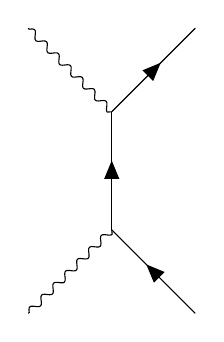
\begin{tikzpicture}
\begin{feynman}
\vertex (i1) ;
\vertex [below right=of i1] (s1);
\vertex [below=of s1] (s2);
\vertex [below left=of s2] (i2);
\vertex [above right=of s1] (f1);
\vertex [below right=of s2] (f2);
\diagram* {
(f2) -- [fermion] (s2) -- [fermion] (s1) -- [fermion] (f1),
(i1) -- [photon] (s1),
(i2) -- [photon] (s2)
};
\end{feynman}
\end{tikzpicture}
\end{center}
Furthermore, $4 m < \Ecm$ which means that a process which creates four electrons/positions is energetically allowed. By charge conservation, no process resulting in an odd number of fermions is possible. Furthermore, charge conservation (given that the photon is uncharged) fixes the only possible four-fermion decay to $\gamma \gamma \to e^{-} e^{-} e^{+} e^{+}$ which is given at lowest order by the diagram,
\begin{center}
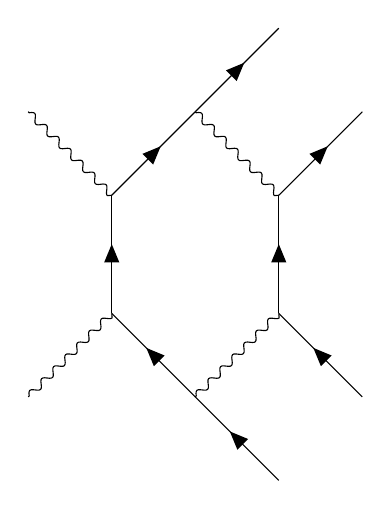
\begin{tikzpicture}
\begin{feynman}
\vertex (i1) ;
\vertex [below right=of i1] (s1);
\vertex [below=of s1] (s2);
\vertex [below left=of s2] (i2);
\vertex [above right=of s1] (f1);
\vertex [below right=of s2] (f2);
\vertex [above right=of f1] (g1);
\vertex [below right=of f2] (g2);
\vertex [below right=of f1] (ss1);
\vertex [above right=of f2] (ss2);
\vertex [above right=of ss1] (e1);
\vertex [below right=of ss2] (e2);
\diagram* {
(f2) -- [fermion] (s2) -- [fermion] (s1) -- [fermion] (f1),
(f1) -- [fermion] (g1),
(g2) -- [fermion] (f2),
(f1) -- [photon] (ss1),
(f2) -- [photon] (ss2),
(i1) -- [photon] (s1),
(i2) -- [photon] (s2),
(e2) -- [fermion] (ss2) -- [fermion] (ss1) -- [fermion] (e1)
};
\end{feynman}
\end{tikzpicture}
\end{center}
We can also produce any even number of bremsstrahlung photons in addition to the one or two electron-positron pairs. These bremsstrahlung photon diagrams give radiative corrections to the total scattering amplitude. 

\subsection{(b)}

There are two tree-level diagrams which contribute to the $\gamma \gamma \to e^{-} e^{+}$ process. These are,
\begin{equation}
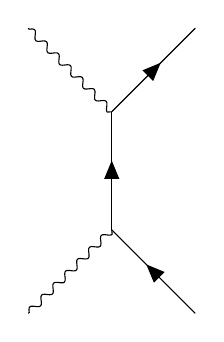
\begin{tikzpicture}
\begin{feynman}
\vertex (i1) ;
\vertex [below right=of i1] (s1);
\vertex [below=of s1] (s2);
\vertex [below left=of s2] (i2);
\vertex [above right=of s1] (f1);
\vertex [below right=of s2] (f2);
\diagram* {
(f2) -- [fermion] (s2) -- [fermion] (s1) -- [fermion] (f1),
(i1) -- [photon] (s1),
(i2) -- [photon] (s2)
};
\end{feynman}
\end{tikzpicture}
\quad \quad \quad
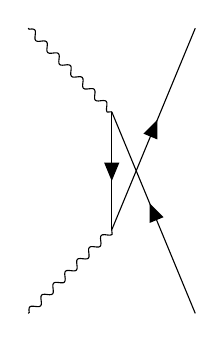
\begin{tikzpicture}
\begin{feynman}
\vertex (i1) ;
\vertex [below right=of i1] (s1);
\vertex [below=of s1] (s2);
\vertex [below left=of s2] (i2);
\vertex [above right=of s1] (f1);
\vertex [below right=of s2] (f2);
\diagram* {
(f2) -- [fermion] (s1) -- [fermion] (s2) -- [fermion] (f1),
(i1) -- [photon] (s1),
(i2) -- [photon] (s2)
};
\end{feynman}
\end{tikzpicture}
\end{equation}
\newcommand{\T}{\mathbf{T}}
I claim that QED is a time-reversal invariant theory. The time-reversal operator is an antiunitary operator $\mathbf{T}$. Spinors transform under time-reversal via\footnote{Peskin and Schroeder chapter 3, Summary of C, P, and T, p. 71},
\[  \T^{-1} \bar{\psi} \psi \T = \bar{\psi} \psi \quad \quad \T^{-1} \bar{\psi} \gamma^\mu \psi \T = (-1)^\mu \bar{\psi} \gamma^\mu \psi \quad \quad \T^{-1} \bar{\psi} \gamma^\mu \partial_\mu \psi \T = - \bar{\psi} \gamma^\mu \partial_\mu \psi \]
Furthermore, we require that $\T^{-1} A_\mu \T = (-1)^\mu A_\mu$ by analogy to classical electromagnetism in which time-reversal reverses currents and therefore reverses magnetic fields but leaves charges and therefore the scalar potential invariant. Therefore, since $\T^{-1} \partial_\mu \T = -(-1)^\mu \partial_\mu$ we have that,
\[ \T^{-1} F_{\mu \nu} \T = \T^{-1} (\partial_\mu A_\nu - \partial_\nu A_\mu) \T = -(-1)^\mu (-1)^\nu F_{\mu \nu} \]
and therefore, the quadratic contractions are left invariant,
\[ \T^{-1} F_{\mu \nu} F^{\mu \nu} \T = [(-1)^\mu (-1)^\nu]^2 F_{\mu \nu} F^{\mu \nu} = F_{\mu \nu} F^{\mu \nu} \]
We now consider the time-reversal of the QED Lagrangian,  
\begin{align*}
\T^{-1} \lagrange_{QED} \T & = - \tfrac{1}{4} \T^{-1} F_{\mu \nu} F^{\mu \nu} \T + \T^{-1} \bar{\psi} (i \gamma^\mu \mathcal{D}_\mu - m) \psi \T
\\
& = - \tfrac{1}{4} F_{\mu \nu} F^{\mu \nu} - i \T^{-1} \bar{\psi} \gamma^\mu \partial_\mu \psi \T - e \T^{-1} A_\mu \T \: \T^{-1} \bar{\psi} \gamma^\mu \psi \T - m \T^{-1} \bar{\psi} \psi \T
\\
& =  - \tfrac{1}{4} F_{\mu \nu} F^{\mu \nu} + i \bar{\psi} \gamma^\mu \partial_\mu - e (-1)^\mu A_\mu (-1)^\mu \bar{\psi} \gamma^\mu \psi - m \bar{\psi} \psi
\\
& = -  \tfrac{1}{4} F_{\mu \nu} F^{\mu \nu} + \bar{\psi} (i \gamma^\mu \mathcal{D}_\mu - m ) \psi = \lagrange_{QED}
\end{align*}
where pulling out the factor of $i$ gives a factor of $-1$ because $\T$ is antiunitary. Since QED is invariant under time-reversal symmetry, the amplitude for a time revered process must be identical to the original up to a possible phase. Therefore, we can use the calculation in Peskin of the scattering cross section for the annihilation process $e^{-} e^{+} \to \gamma \gamma$ to calculate the cross section for pair production $\gamma \gamma \to e^{-} e^{+}$. The differential cross section for the former process is\footnote{Peskin and Schroeder chapter 5, Pair Annihilation into Photons, p. 168},
\[ \deriv{\sigma}{(\cos{\theta})} = \frac{2 \pi \alpha^2}{s} \left( \frac{E}{p} \right) \left[ \frac{E^2 + 2m^2 + p^2 \cos^2{\theta}}{m^2 + p^2 \sin^2{\theta}} - \frac{2m^4}{(m^2 + p^2 \sin^2{\theta})^2} \right] \]
where $E$ is the energy of one photon, $s = \Ecm^2 = 4E^2$ and $p^2 = E^2 - m^2$ is the momentum of one of the electrons. However, it is the amplitude not the cross section which is invariant under time reversal because the incoming and outgoing states are distinct. Therefore, we need to modify the prefactor to account for the difference in incoming particles. In the center of mass frame,
\[ \left( \deriv{\sigma}{\Omega} \right)_{\mathrm{CM}} = \frac{1}{2 E_{\mathcal{A}} 2 E_{\mathcal{B}} |v_{\mathcal{A}} - v_{\mathcal{B}} | } \frac{|\vec{p}_1|}{(2 \pi)^2 4 \Ecm} | \mathcal{M} |^2 \]
where $\mathcal{A}$ and $\mathcal{B}$ refer to the incoming particles and $\vec{p}_1$ is the vector momentum of one of the outgoing particles. We can restrict to the case that the two incoming particles and the two outgoing particles are indistinguishable. Then, $2E_{\mathcal{A}} = 2 E_{\mathcal{B}} = \Ecm$ and $v_{\mathcal{A}} = v_{\mathcal{B}} = \frac{2p}{\Ecm}$ where $p = |\vec{p}_{\mathcal{A}}| = |\vec{p}_{\mathcal{B}}|$. This implies that $|v_{\mathcal{A}} - v_{\mathcal{B}}| = 4 \frac{p}{\Ecm}$.  Thus, we can write,
\[
\left( \deriv{\sigma}{\Omega} \right)_{\mathrm{CM}} = \frac{|\mathcal{M}|^2}{64 \pi^2 \Ecm^2} \left( \frac{p'}{p} \right)
\]
where $p' = |\vec{p}_1|$ is the magnitude of the final momentum. 
Therefore, the ratio of the cross sections for these two processes is,
\[ \frac{\sigma(\gamma \gamma \to e^{-} e^{+})}{\sigma(e^{-} e^{+} \to \gamma \gamma)} = \left( \frac{|\vec{p}_e|}{|\vec{p}_\gamma|} \right)^2 = \left( \frac{p}{E} \right)^2 = \frac{E^2 - m^2}{E^2} = 1 - \left( \frac{2m}{\Ecm} \right)^2 \]
This factor gives a cutoff at the threshold for electron-positron pair production. Therefore, the cross section for $\gamma \gamma \to e^{-} e^{+}$ becomes,
\[ \deriv{\sigma}{(\cos{\theta})} = \frac{2 \pi \alpha^2}{s} \left( \frac{p}{E} \right) \left[ \frac{E^2 + 2m^2 + p^2 \cos^2{\theta}}{m^2 + p^2 \sin^2{\theta}} - \frac{2m^4}{(m^2 + p^2 \sin^2{\theta})^2} \right] \]
To find the total cross section for the process, we integrate over the sphere of scattering angles,
\[ 
\sigma = \int_{-1}^{1} \deriv{\sigma}{(\cos{\theta})} \d{(\cos{\theta})} 
\]
Using the given parameters, $\Ecm = 2.2 \MeV$ and $m = 0.511 \MeV$ we have, $E = 1.1 \MeV$ and $p = 0.97 \MeV$. Integrating the above expression for the differential cross section numerically, we arrive at,
\[ \sigma = 313 \GeV^{-2} \]
in our mass-dimension units. We can convert to physical units by noting that,
\[ \frac{\hbar^2 c^2}{\mathrm{GeV}^2} = 0.3894 \, \mathrm{mb} \]
and therefore, 
\[ \sigma =  0.122 \, \mathrm{b} \]
\section{}

\subsection{(a)}

Consider the $D = 1 + 1$ dimensional free Dirac Lagrangian,
\[ \lagrange_0 = \bar{\psi} ( i \gamma^\mu \partial_\mu - m) \psi \]
where $\gamma^0 = \sigma^1$ and $\gamma^1 = i \sigma^2$ such that $\{ \gamma^\mu, \gamma^\nu \} = 2 \eta^{\mu \nu}$. 
\bigskip\\
\subsubsection{Plane Wave Solutions}
The Dirac equation in $D = 1 + 1$ dimensions derived from the above Lagrangian has exactly the same form as in ordinary $D = 3 + 1$ dimensions replacing bispinors with ordinary two-component spinors and using the above expressions for the two gamma matrices. We want to consider solutions to the classical equation of motion of the form $\psi = u^s e^{ \mp i p x}$. Therefore,
\[ \gamma^\mu p_\mu u_p = \pm m u_p \implies 
\begin{pmatrix}
\mp m & p^0 - p^1 
\\
p^0 + p^1 & \mp m
\end{pmatrix} u_p = 0 \] 
Which only has nontrivial solutions when the determinant is zero i.e. $(p^0 + p^1)(p^0 - p^1) - m^2 = 0$ or equivalently, $p^2 = m^2$. The nontrivial solutions to this matrix equation are,
\[ u_p = 
\begin{pmatrix}
\sqrt{p^0 - p^1}
\\
\sqrt{p^0 + p^1}
\end{pmatrix}  \quad \text{and} \quad
v_p = 
\begin{pmatrix}
\sqrt{p^0 - p^1}
\\
-\sqrt{p^0 + p^1}
\end{pmatrix} \]
for the positive and negative frequency modes respectively. These satisfy,  
\[ \bar{u}_p u_p = 2 m \quad \text{and} \quad \bar{v}_p v_p = -2 m\]
\[ u^\dagger_p u_p = 2 p^0 \quad \text{and} \quad v^\dagger_p v_p = -2 p^0\]
and similarly,
\[ u_p \bar{u}_p = \slashed{p} + m \quad \text{and} \quad v_p \bar{v}_p = \slashed{p} - m\]

\subsubsection{The Mode Expansion}

In terms of these wave-function factors I propose the following form of the mode expansion,
\[ \psi(x) = \int \frac{\d{p^1}}{2 \pi} \frac{1}{\sqrt{2 p^0}} \left( \a_p u_p e^{-i p \cdot x} + \bdag_p v_p e^{i p \cdot x} \right) \]
where the creation and annihilation operators are defined to satisfy,
\[ \{ \a_p, \adag_q \} = 2 \pi \: \delta(p^1 - q^1) \quad \quad \{ \b_p, \bdag_q \} = 2 \pi \: \delta(p^1 - q^1) \]
We need to check that these definitions satisfy the equal-time canonical anti-commutation relations,
\begin{align*}
\{ \psi_{\alpha}(x), \psi_\beta(y) \} & = \{ \psi_{\alpha}^\dagger(x), \psi_{\beta}^\dagger(y) \} =  0 
\\
\{ \psi_{\alpha}(x), \psi_{\beta}^\dagger(y) \} & = \delta_{\alpha \beta} \delta(x^1 - y^1)
\end{align*}
where the second is equivalent to the canonical anti-commutation relations for the conjugate momentum, 
\[\Pi = i \bar{\psi} \gamma^0 = i \psi \implies \{ \psi_\alpha(x), \Pi_{\beta}(y) \} = i \delta_{\alpha \beta} \delta(x^1 - y^1) \]
The first of the commutation relations is obvious because $\a$ and $\bdag$ commute and all operators commute with themselves. Therefore, for $x^0 = y^0$, consider,
\begin{align*}
\{ \psi_{\alpha}(x), \bar{\psi}_{\beta}(y) \} & = \frac{1}{(2 \pi)^2} \int_{-\infty}^{\infty} \frac{\d{p^1} \d{q^1}}{\sqrt{4 p^0 q^0}} \left[ \{ \a_p , \adag_p \} (u_p)_{\alpha} (\bar{u}_q)_{\beta} e^{-i p \cdot x + i q \cdot y} + \{ \bdag_p, \b_q \} (v_p)_{\alpha} (\bar{v}_q)_{\beta} e^{i p \cdot x - i q \cdot y} \right] 
\\
& = \frac{1}{2 \pi } \int_{-\infty}^{\infty} \frac{\d{p^1}}{2 p^0} \left[ (\slashed{p} + m)_{\alpha \beta} e^{-i p \cdot (x - y)} + (\slashed{p} - m)_{\alpha \beta} e^{i p \cdot (x - y)} \right] 
\\
& = \frac{1}{2 \pi } \int_{-\infty}^{\infty} \frac{\d{p^1}}{2 p^0} \left[ \slashed{p}_{\alpha \beta} \left( e^{-i p \cdot (x - y)} + e^{i p \cdot (x - y)} \right) + m \delta_{\alpha \beta} \left( e^{-i p \cdot (x - y)} - e^{i p \cdot (x - y)} \right) \right] 
\\
& = \frac{1}{4 \pi } \int_{-\infty}^{\infty} \d{p^1} \left[ \left( \gamma^0 - \frac{p^1}{p^0} \gamma^1 \right)_{\alpha \beta} \left( e^{-i p \cdot (x - y)} + e^{i p \cdot (x - y)} \right) + m \delta_{\alpha \beta} \left( e^{-i p \cdot (x - y)} - e^{i p \cdot (x - y)} \right) \right] 
\\
& = \gamma^0_{\alpha \beta} \delta(x^1 - y^1)
\end{align*} 
where all but the first term integrate to zero because both $e^{-i p \cdot (x - y)} - e^{i p \cdot (x - y)}$ and $p^1 (e^{-i p \cdot (x - y)} + e^{i p \cdot (x - y)})$ are odd functions. Therefore, my normalization and wave-function factors in the mode expansion are correct. 

\subsection{(b)}

Now consider the interacting $1+1$-dimensional Yukawa type theory with Lagrangian,
\[ \lagrange = \bar{\psi} \left( i \slashed{\partial} - m \right) \psi + \tfrac{1}{2} \partial_\mu \psi \partial^\mu \psi - \tfrac{1}{2} M^2 \phi^2 - M \phi \bar{\psi} \Gamma \psi + \mathrm{ c.t. }\]
where we have a vertex interaction,
\[ \Gamma = g_e \mathrm{1} + g_o i \gamma^5 \]
where $\gamma^5 = \gamma^0 \gamma^1$. 
\bigskip\\
The previous problem gives us enough information to write down the Feynman rules,
\subsubsection{Feynman Rules}
\begin{equation*}
\feynmandiagram [small, baseline=(d.base), horizontal=d to b] {
a -- [fermion] b -- [fermion] c,
b -- [scalar] d
};
= -i M \Gamma
\end{equation*}
\begin{itemize}
\item Each internal meson line gives a factor of $\frac{i}{p^2 - M^2 + i \epsilon}$
\item Each internal nucleon line gives a factor of $\frac{i (\slashed{p} + m)}{p^2 - m^2 + i \epsilon}$
\item Each vertex gives a factor of $(-i M \Gamma)(2 \pi) \delta^2(\sum p)$
\item Integrate over all undetermined momenta with measure $\int \frac{\dn{2}{p}}{(2\pi)^2}$
\item Each incoming nucleon gives a factor of $u_p$ while an outgoing nucleon gives a factor of $\bar{u}_p$.
\item Each incoming anti-nucleon gives a factor of $\bar{v}_p$ while an outgoing nucleon gives a factor of $v_p$.
\end{itemize}
\subsubsection{$\psi \psi \to \psi \psi$ scattering}
The scattering process $\psi \psi \to \psi \psi$ is given by two diagrams at tree-level,
\begin{equation*}
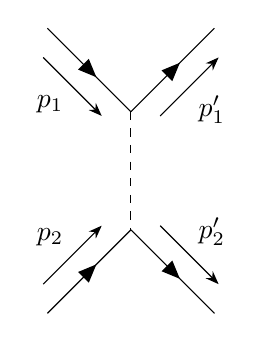
\begin{tikzpicture}
\begin{feynman}
\vertex (i1) ;
\vertex [below right=of i1] (s1);
\vertex [below=of s1] (s2);
\vertex [below left=of s2] (i2);
\vertex [above right=of s1] (f1);
\vertex [below right=of s2] (f2);
\diagram* {
(i1) -- [fermion, momentum'=\(p_1\)] (s1) -- [fermion, momentum'=\(p_1'\)] (f1),
(s1) -- [scalar] (s2),
(i2) -- [fermion, momentum=\(p_2\)] (s2) -- [fermion, momentum=\(p_2'\)] (f2)
};
\end{feynman}
\end{tikzpicture}
\quad \quad \quad
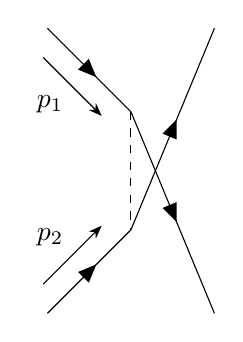
\begin{tikzpicture}
\begin{feynman}
\vertex (i1) ;
\vertex [below right=of i1] (s1);
\vertex [below=of s1] (s2);
\vertex [below left=of s2] (i2);
\vertex [above right=of s1] (f1);
\vertex [below right=of s2] (f2);
\diagram* {
(i1) -- [fermion, momentum'=\(p_1\)] (s1) -- [fermion] (f2),
(s1) -- [scalar] (s2),
(i2) -- [fermion, momentum=\(p_2\)] (s2) -- [fermion] (f1)
};
\end{feynman}
\end{tikzpicture}
\end{equation*}
Therefore, the tree-level amplitude for this process is,
\begin{align*}
i\mathcal{M} & = (\bar{u}_{p_1'} (-i M \Gamma) u_{p_1}) \frac{i}{t - M^2 + i \epsilon} (\bar{u}_{p_2'} (-i M \Gamma) u_{p_2}) - (\bar{u}_{p_1'} (-i M \Gamma) u_{p_2}) \frac{i}{u - M^2 + i \epsilon} (\bar{u}_{p_2'} (-i M \Gamma) u_{p_1}) 
\\
& = -i(\bar{u}_{p_1'} \Gamma u_{p_1}) \frac{M^2}{t - M^2 + i \epsilon} (\bar{u}_{p_2'} \Gamma u_{p_2}) + i (\bar{u}_{p_1'} \Gamma u_{p_2}) \frac{M^2}{u - M^2 + i \epsilon} (\bar{u}_{p_2'} \Gamma u_{p_1}) 
\end{align*}
where the relative minus sign comes from swapping outgoing fermion lines. 


\subsection{(c)}

In the limit $M \to \infty$ the $\phi$-meson can be integrated out of the theory if we only consider asymptotic states with $\psi$ and $\bar{\psi}$ particles. First, we consider an alternative theory which will turn out to give the $M \to \infty$ limit. 
\subsubsection{The Quadratic $\psi$ Theory}

Consider the Lagrangian,
\[ \lagrange' = \bar{\psi} (i \slashed{\partial} - m) \psi + \tfrac{1}{2} ( \bar{\psi} \Gamma' \psi) (\bar{\psi} \Gamma' \psi) + \mathrm{ c.t. } \]
We need to determine the Feynman rules of this theory. This theory is the free Dirac field in $1 + 1$-dimensions plus an interaction Hamiltonian of the form,
\[ \mathcal{H}_{\mathrm{int}} = - \tfrac{1}{2} ( \bar{\psi} \Gamma' \psi) (\bar{\psi} \Gamma' \psi) - \mathrm{ c.t. } \]
Therefore, the following term appears in the Dyson series,
\[ \tfrac{i}{2} ( \bar{\psi} \Gamma' \psi) (\bar{\psi} \Gamma' \psi) \]
To determine the Feynman rules, consider the four-point function where I now use creation and annihilation operators with relativistic normalization, 
\begin{align*}
\bra{0} \a_{p_2'} \a_{p_1'} \tfrac{i}{2} ( \bar{\psi} \Gamma' \psi) (\bar{\psi} \Gamma' \psi)\adag_{p_1} \adag_{p_2} \ket{0} 
& =
\contraction{}{ \a_{p_2'}}{ \a_{p_1'}\tfrac{i}{2} ( }{\bar{\psi}}
\contraction[2ex]{\a_{p_2'} }{ \a_{p_1'} }{ \tfrac{i}{2} ( \bar{\psi} \Gamma' \psi) (} {\bar{\psi}} 
\contraction{\a_{p_2'} \a_{p_1'} \tfrac{i}{2} ( \bar{\psi} \Gamma'}{ \psi}{) (\bar{\psi} \Gamma' \psi)}{\adag}
\contraction[2ex]{\a_{p_2'} \a_{p_1'} \tfrac{i}{2} ( \bar{\psi} \Gamma' \psi) (\bar{\psi} \Gamma'}{ \psi }{)\adag_{p_1}}{ \adag}
\a_{p_2'} \a_{p_1'} \tfrac{i}{2} ( \bar{\psi} \Gamma' \psi) (\bar{\psi} \Gamma' \psi)\adag_{p_1} \adag_{p_2}
\\
& +  
\contraction{\a_{p_2'}}{ \a_{p_1'}}{\tfrac{i}{2} ( }{\bar{\psi}}
\contraction[2ex]{}{ \a_{p_2'} }{ \a_{p_1'} \tfrac{i}{2} ( \bar{\psi} \Gamma' \psi) (} {\bar{\psi}} 
\contraction{\a_{p_2'} \a_{p_1'} \tfrac{i}{2} ( \bar{\psi} \Gamma'}{ \psi}{) (\bar{\psi} \Gamma' \psi)}{\adag}
\contraction[2ex]{\a_{p_2'} \a_{p_1'} \tfrac{i}{2} ( \bar{\psi} \Gamma' \psi) (\bar{\psi} \Gamma'}{ \psi }{)\adag_{p_1}}{ \adag}
\a_{p_2'} \a_{p_1'} \tfrac{i}{2} ( \bar{\psi} \Gamma' \psi) (\bar{\psi} \Gamma' \psi)\adag_{p_1} \adag_{p_2} 
\\
& + 
\contraction{}{ \a_{p_2'}}{ \a_{p_1'}\tfrac{i}{2} ( }{\bar{\psi}}
\contraction[2ex]{\a_{p_2'} }{ \a_{p_1'} }{ \tfrac{i}{2} ( \bar{\psi} \Gamma' \psi) (} {\bar{\psi}} 
\contraction{\a_{p_2'} \a_{p_1'} \tfrac{i}{2} ( \bar{\psi} \Gamma'}{ \psi}{) (\bar{\psi} \Gamma' \psi) \adag_{p_1}}{\adag}
\contraction[2ex]{\a_{p_2'} \a_{p_1'} \tfrac{i}{2} ( \bar{\psi} \Gamma' \psi) (\bar{\psi} \Gamma'}{ \psi }{)}{\adag}
\a_{p_2'} \a_{p_1'} \tfrac{i}{2} ( \bar{\psi} \Gamma' \psi) (\bar{\psi} \Gamma' \psi)\adag_{p_1} \adag_{p_2} 
\\
& +  
\contraction{\a_{p_2'}}{ \a_{p_1'}}{\tfrac{i}{2} ( }{\bar{\psi}}
\contraction[2ex]{}{ \a_{p_2'} }{ \a_{p_1'} \tfrac{i}{2} ( \bar{\psi} \Gamma' \psi) (} {\bar{\psi}} 
\contraction{\a_{p_2'} \a_{p_1'} \tfrac{i}{2} ( \bar{\psi} \Gamma'}{ \psi}{) (\bar{\psi} \Gamma' \psi) \adag_{p_1}}{\adag}
\contraction[2ex]{\a_{p_2'} \a_{p_1'} \tfrac{i}{2} ( \bar{\psi} \Gamma' \psi) (\bar{\psi} \Gamma'}{ \psi }{)}{\adag}
\a_{p_2'} \a_{p_1'} \tfrac{i}{2} ( \bar{\psi} \Gamma' \psi) (\bar{\psi} \Gamma' \psi)\adag_{p_1} \adag_{p_2} 
\\
& = -\tfrac{i}{2} ( \bar{u}_{p_2'} \Gamma' u_{p_1}) (\bar{u}_{p_1'} \Gamma' u_{p_2}) + \tfrac{i}{2} ( \bar{u}_{p_1'} \Gamma' u_{p_1}) (\bar{u}_{p_2'} \Gamma' u_{p_2})
\\
& + \tfrac{i}{2} ( \bar{u}_{p_2'} \Gamma' u_{p_2}) (\bar{u}_{p_1'} \Gamma' u_{p_1}) - \tfrac{i}{2} ( \bar{u}_{p_1'} \Gamma' u_{p_2}) (\bar{u}_{p_2'} \Gamma' u_{p_1})
\\
& = i ( \bar{u}_{p_1'} \Gamma' u_{p_1}) (\bar{u}_{p_2'} \Gamma' u_{p_2}) - i ( \bar{u}_{p_1'} \Gamma' u_{p_2}) (\bar{u}_{p_2'} \Gamma' u_{p_1})
\end{align*}
This is exactly the amplitude I calculated above in the limit $M \to \infty$ if we take $\Gamma' = \Gamma$. Furthermore, 
we can compute the four-point interaction term for $\bar{\psi} \bar{\psi} \to \bar{\psi} \bar{\psi}$ and for $\psi \bar{\psi} \to \psi \bar{\psi}$. The results are given below. For $\bar{\psi} \bar{\psi} \to \bar{\psi} \bar{\psi}$ scattering we get,
\begin{align*}
\bra{0} \b_{p_2'} \b_{p_1'} \tfrac{i}{2} ( \bar{\psi} \Gamma' \psi) (\bar{\psi} \Gamma' \psi)\bdag_{p_1} \bdag_{p_2} \ket{0} 
& =
\contraction[3ex]{}{ \b_{p_2'} }{ \b_{p_1'}\tfrac{i}{2} ( \bar{\psi} \Gamma'}{ \psi }
\contraction[2ex]{\b_{p_2'} }{ \b_{p_1'} }{ \tfrac{i}{2} ( \bar{\psi} \Gamma' \psi) ( \bar{\psi} \Gamma' }{ \psi } 
\contraction{\b_{p_2'} \b_{p_1'} \tfrac{i}{2} (}{ \bar{\psi} }{ \Gamma' \psi ) (\bar{\psi} \Gamma' \psi)}{\bdag}
\contraction[4ex]{\b_{p_2'} \b_{p_1'} \tfrac{i}{2} ( \bar{\psi} \Gamma' \psi) (}{\bar{\psi} }{ \Gamma' \psi )\bdag_{p_1}}{ \bdag}
\b_{p_2'} \b_{p_1'} \tfrac{i}{2} ( \bar{\psi} \Gamma' \psi) (\bar{\psi} \Gamma' \psi)\bdag_{p_1} \bdag_{p_2}
\\
& +  
\contraction[3ex]{ \b_{p_2'} }{ \b_{p_1'} }{\tfrac{i}{2} ( \bar{\psi} \Gamma'}{ \psi }
\contraction[2ex]{}{\b_{p_2'} }{ \b_{p_1'} \tfrac{i}{2} ( \bar{\psi} \Gamma' \psi) ( \bar{\psi} \Gamma' }{ \psi } 
\contraction{\b_{p_2'} \b_{p_1'} \tfrac{i}{2} (}{ \bar{\psi} }{ \Gamma' \psi ) (\bar{\psi} \Gamma' \psi)}{\bdag}
\contraction[4ex]{\b_{p_2'} \b_{p_1'} \tfrac{i}{2} ( \bar{\psi} \Gamma' \psi) (}{\bar{\psi} }{ \Gamma' \psi )\bdag_{p_1}}{ \bdag}
\b_{p_2'} \b_{p_1'} \tfrac{i}{2} ( \bar{\psi} \Gamma' \psi) (\bar{\psi} \Gamma' \psi)\bdag_{p_1} \bdag_{p_2}
\\
& + 
\contraction[3ex]{}{ \b_{p_2'} }{ \b_{p_1'}\tfrac{i}{2} ( \bar{\psi} \Gamma'}{ \psi }
\contraction[2ex]{\b_{p_2'} }{ \b_{p_1'} }{ \tfrac{i}{2} ( \bar{\psi} \Gamma' \psi) ( \bar{\psi} \Gamma' }{ \psi } 
\contraction{\b_{p_2'} \b_{p_1'} \tfrac{i}{2} ( \bar{\psi}  \Gamma'  \psi  ) ( }{ \bar{\psi} }{ \Gamma' \psi)}{\bdag}
\contraction[4ex]{\b_{p_2'} \b_{p_1'} \tfrac{i}{2} ( }{ \bar{\psi} }{ \Gamma' \psi) ( \bar{\psi}  \Gamma' \psi )\bdag_{p_1} }{ \bdag}
\b_{p_2'} \b_{p_1'} \tfrac{i}{2} ( \bar{\psi} \Gamma' \psi) (\bar{\psi} \Gamma' \psi)\bdag_{p_1} \bdag_{p_2}
\\
& +  
\contraction[3ex]{ \b_{p_2'} }{ \b_{p_1'} }{\tfrac{i}{2} ( \bar{\psi} \Gamma'}{ \psi }
\contraction[2ex]{}{\b_{p_2'} }{ \b_{p_1'} \tfrac{i}{2} ( \bar{\psi} \Gamma' \psi) ( \bar{\psi} \Gamma' }{ \psi } 
\contraction{\b_{p_2'} \b_{p_1'} \tfrac{i}{2} ( \bar{\psi}  \Gamma'  \psi  ) ( }{ \bar{\psi} }{ \Gamma' \psi)}{\bdag}
\contraction[4ex]{\b_{p_2'} \b_{p_1'} \tfrac{i}{2} ( }{ \bar{\psi} }{ \Gamma' \psi) ( \bar{\psi}  \Gamma' \psi )\bdag_{p_1} }{ \bdag}
\b_{p_2'} \b_{p_1'} \tfrac{i}{2} ( \bar{\psi} \Gamma' \psi) (\bar{\psi} \Gamma' \psi)\bdag_{p_1} \bdag_{p_2}
\\
& = -\tfrac{i}{2} ( \bar{v}_{p_1} \Gamma' v_{p_2'}) (\bar{v}_{p_2} \Gamma' v_{p_1'}) + \tfrac{i}{2} ( \bar{v}_{p_1} \Gamma' v_{p_1'}) (\bar{v}_{p_2} \Gamma' v_{p_2'})
\\
& + \tfrac{i}{2} ( \bar{v}_{p_2} \Gamma' v_{p_2'}) (\bar{v}_{p_1} \Gamma' v_{p_1'}) - \tfrac{i}{2} ( \bar{v}_{p_2} \Gamma' v_{p_1'}) (\bar{v}_{p_1} \Gamma' v_{p_2'})
\\
& = i ( \bar{v}_{p_1} \Gamma' v_{p_1'}) (\bar{v}_{p_2} \Gamma' v_{p_2'}) - i ( \bar{v}_{p_1} \Gamma' v_{p_2'}) (\bar{v}_{p_2} \Gamma' v_{p_1'})
\end{align*}
Finally, for $\psi \bar{\psi} \to \psi \bar{\psi}$ scattering, we get,
\begin{align*}
\bra{0} \b_{p_2'} \a_{p_1'} \tfrac{i}{2} ( \bar{\psi} \Gamma' \psi) (\bar{\psi} \Gamma' \psi)\adag_{p_1} \bdag_{p_2} \ket{0} 
& =
\contraction[2ex]{}{\b_{p_2'}}{ \a_{p_1'} \tfrac{i}{2} ( \bar{\psi} \Gamma' \psi) (\bar{\psi} \Gamma'}{ \psi}
\contraction{\b_{p_2'} }{ \a_{p_1'} }{ \tfrac{i}{2} ( \bar{\psi} \Gamma' \psi) (} {\bar{\psi}} 
\contraction[2ex]{\b_{p_2'} \a_{p_1'} \tfrac{i}{2} ( \bar{\psi} \Gamma'}{ \psi}{) (\bar{\psi} \Gamma' \psi)}{\adag}
\contraction[3ex]{\b_{p_2'} \a_{p_1'} \tfrac{i}{2} ( }{ \bar{\psi} }{ \Gamma' \psi) ( \bar{\psi}  \Gamma' \psi )\adag_{p_1} }{ \bdag}
\b_{p_2'} \a_{p_1'} \tfrac{i}{2} ( \bar{\psi} \Gamma' \psi) (\bar{\psi} \Gamma' \psi)\adag_{p_1} \bdag_{p_2}
\\
& +  
\contraction[2ex]{}{\b_{p_2'}}{ \a_{p_1'} \tfrac{i}{2} ( \bar{\psi} \Gamma'}{ \psi}
\contraction{\b_{p_2'} }{ \a_{p_1'} }{ \tfrac{i}{2} ( \bar{\psi} \Gamma' \psi) (} {\bar{\psi}} 
\contraction[2ex]{\b_{p_2'} \a_{p_1'} \tfrac{i}{2} ( \bar{\psi} \Gamma' \psi) (\bar{\psi} \Gamma'}{ \psi}{)}{\adag}
\contraction[3ex]{\b_{p_2'} \a_{p_1'} \tfrac{i}{2} ( }{ \bar{\psi} }{ \Gamma' \psi) ( \bar{\psi}  \Gamma' \psi )\adag_{p_1} }{ \bdag}
\b_{p_2'} \a_{p_1'} \tfrac{i}{2} ( \bar{\psi} \Gamma' \psi) (\bar{\psi} \Gamma' \psi)\adag_{p_1} \bdag_{p_2}
\\
& + 
\contraction[2ex]{}{\b_{p_2'}}{ \a_{p_1'} \tfrac{i}{2} ( \bar{\psi} \Gamma' \psi) (\bar{\psi} \Gamma'}{ \psi}
\contraction{\b_{p_2'} }{ \a_{p_1'} }{ \tfrac{i}{2} (}{ \bar{\psi} } 
\contraction[2ex]{\b_{p_2'} \a_{p_1'} \tfrac{i}{2} ( \bar{\psi} \Gamma'}{ \psi}{) (\bar{\psi} \Gamma' \psi)}{\adag}
\contraction[3ex]{\b_{p_2'} \a_{p_1'} \tfrac{i}{2} ( \bar{\psi} \Gamma' \psi) (}{ \bar{\psi} }{ \Gamma' \psi )\adag_{p_1} }{ \bdag}
\b_{p_2'} \a_{p_1'} \tfrac{i}{2} ( \bar{\psi} \Gamma' \psi) (\bar{\psi} \Gamma' \psi)\adag_{p_1} \bdag_{p_2}
\\
& +  
\contraction[2ex]{}{\b_{p_2'}}{ \a_{p_1'} \tfrac{i}{2} ( \bar{\psi} \Gamma'}{ \psi}
\contraction{\b_{p_2'} }{ \a_{p_1'} }{ \tfrac{i}{2} (}{ \bar{\psi} } 
\contraction{\b_{p_2'} \a_{p_1'} \tfrac{i}{2} ( \bar{\psi} \Gamma' \psi) (\bar{\psi} \Gamma'}{ \psi}{)}{\adag}
\contraction[2ex]{\b_{p_2'} \a_{p_1'} \tfrac{i}{2} ( \bar{\psi} \Gamma' \psi) (}{ \bar{\psi} }{ \Gamma' \psi )\adag_{p_1} }{ \bdag}
\b_{p_2'} \a_{p_1'} \tfrac{i}{2} ( \bar{\psi} \Gamma' \psi) (\bar{\psi} \Gamma' \psi)\adag_{p_1} \bdag_{p_2}
\\
& = \tfrac{i}{2} ( \bar{v}_{p_2} \Gamma' u_{p_1}) (\bar{u}_{p_1'} \Gamma' v_{p_2'}) - \tfrac{i}{2} ( \bar{v}_{p_2} \Gamma' v_{p_2'}) (\bar{u}_{p_1'} \Gamma' u_{p_1})
\\
& - \tfrac{i}{2} ( \bar{u}_{p_1'} \Gamma' u_{p_1}) (\bar{v}_{p_2} \Gamma' v_{p_2'}) + \tfrac{i}{2} ( \bar{u}_{p_1'} \Gamma' v_{p_2'}) (\bar{v}_{p_2} \Gamma' u_{p_1})
\\
& = i ( \bar{v}_{p_2} \Gamma' u_{p_1}) (\bar{u}_{p_1'} \Gamma' v_{p_2'}) - i ( \bar{v}_{p_2} \Gamma' v_{p_2'}) (\bar{u}_{p_1'} \Gamma' u_{p_1})
\end{align*}
These are exactly the results we would expect from the two tree-level diagrams from each process in the Yukawa theory with the limit $M \to \infty$ taking $\Gamma' = \Gamma$.


\subsection{(d)}
To compute the scattering cross section, we must first find the $1+1$-dimensional equivalent of the formula for the cross-section in terms of the scattering amplitudes.

\subsubsection{The $1+1$-Dimensional Scattering Cross Section}

Following Peskin's conventions, to compute physical scattering amplitudes, we need to construct wavepackets for the two incoming particles of the form,
\[ \ket{\phi_{\mathcal{A}} \phi_{\mathcal{B}}}_{\mathrm{in}} = \int \frac{\d{k_{\mathcal{A}}}}{2 \pi} \int \frac{\d{k_{\mathcal{B}}}}{2 \pi} \frac{ \phi_\mathcal{A}(k_\mathcal{A}) \phi_{\mathcal{B}}(k_{\mathcal{B}}) }{ \sqrt{ (2 E_\mathcal{A}) (2 E_{\mathcal{B}}) }} \ket{k_\mathcal{A} k_{\mathcal{B}}}_{\mathrm{in}} \]
The overlap between in and out states gives us the scattering matrix,
\[ {}_{\mathrm{out}} \inner{p_1 p_2}{k_\mathcal{A} k_{\mathcal{B}}}_{\mathrm{in}} = \bra{p_1 p_2} S \ket{k_\mathcal{A} k_{\mathcal{B}}} \]
We will write the scattering matrix as $S = \mathrm{1} + i T$ to subtract off the trivial non-interacting processes. Furthermore, we know that this amplitude takes the general form,
\[ \mathcal{\mathcal{A}}_{i \to f} = \bra{p_1 p_2} iT \ket{k_\mathcal{A} k_{\mathcal{B}}} = (2 \pi )^2 \delta^2(p_{\mathrm{tot}}) \: i \mathcal{M} \] 
Following Peskin, we define the probability for scattering into a small range of possible momenta,
\[ \mathcal{P}(\mathcal{A} \mathcal{B} \to 1,2) = \left( \prod_{f} \frac{\d{p_f}}{2 \pi} \frac{1}{2 E_f} \right) | \bra{p_1 p_2} iT \ket{\phi_\mathcal{A} \phi_{\mathcal{B}}} |^2 \] 
Because there is only one spatial dimension, there is no need to integrate over the impact parameter. Therefore, we define the ``cross section'' as,
\[ \d{\sigma} = \frac{\d{N}}{N_{\mathcal{A}} N_{\mathcal{B}}} \]
where $N_{\mathcal{A}}$ and $N_{\mathcal{B}}$ are the number of $\mathcal{A}$ and $\mathcal{B}$ particles respectively and $\d{N}$ is the number of events in an a given momentum range given by, 
\[ \d{N} = N_{\mathcal{A}} N_{\mathcal{B}} \mathcal{P} \]
Combining these terms,
\begin{align*}
\d{\sigma} = \mathcal{P} = \left( \prod_{f} \frac{\d{p_f}}{2 \pi} \frac{1}{2 E_f} \right) \left| \int \frac{\d{k_{\mathcal{A}}} \d{k_{\mathcal{B}}}}{(2 \pi)^2} \frac{ \phi_\mathcal{A}(k_\mathcal{A}) \phi_{\mathcal{B}}(k_{\mathcal{B}}) }{ \sqrt{ (2 E_\mathcal{A}) (2 E_\mathcal{B}) }} (2 \pi)^2 \delta^2 \left(\sum_{i} k_i -  \sum p_f \right) \mathcal{M}(\{ k_i \} \to \{p_f \}) \right|^2
\end{align*} 
Consider the integral, 
\begin{align*}
\int & \frac{\d{k_{\mathcal{A}}} \d{k_{\mathcal{B}}}}{(2 \pi)^2} \frac{ \phi_\mathcal{A}(k_\mathcal{A}) \phi_{\mathcal{B}}(k_{\mathcal{B}}) }{ \sqrt{ (2 E_\mathcal{A}) (2 E_\mathcal{B}) }} (2 \pi)^2 \delta^2 \left(\sum_{i} k_i -  \sum p_f \right) \mathcal{M}(\{ k_i \} \to \{p_f \}) 
\\
& = \int \frac{\d{k_{\mathcal{A}}} \d{k_{\mathcal{B}}}}{(2 \pi)^2} \frac{ \phi_\mathcal{A}(k_\mathcal{A}) \phi_{\mathcal{B}}(k_{\mathcal{B}}) }{ \sqrt{ (2 E_\mathcal{A}) (2 E_\mathcal{B}) }} (2 \pi)^2 \delta \left(k_{\mathcal{A}} + k_{\mathcal{B}} -  \sum p_f \right) \delta \left(E_{\mathcal{A}} + E_{\mathcal{B}} -  \sum p_f \right) \mathcal{M}(\{ k_i \} \to \{p_f \}) 
\\
& = \frac{ \phi_\mathcal{A}(k_\mathcal{A}) \phi_{\mathcal{B}}(k_{\mathcal{B}}) }{ \sqrt{ (2 E_\mathcal{A}) (2 E_\mathcal{B}) }} \mathcal{M}(\{ k_i \} \to \{p_f \}) \bigg|_{(k_{\mathcal{A}} + k_{\mathcal{B}} = \sum p_f)} \frac{1}{| \deriv{}{k_{\mathcal{A}}} (E_{\mathcal{A}} + E_{\mathcal{B}})|_{(k_{\mathcal{A}} + k_{\mathcal{B}} = \sum p_f)} |} 
\\
& = \frac{ \phi_\mathcal{A}(k_\mathcal{A}) \phi_{\mathcal{B}}(k_{\mathcal{B}}) }{ \sqrt{ (2 E_\mathcal{A}) (2 E_\mathcal{B}) }} \frac{1}{\left| \frac{k_{\mathcal{A}}}{E_{\mathcal{A}}} - \frac{k_{\mathcal{B}}}{E_{\mathcal{B}}} \right|}  \mathcal{M}(\{ k_i \} \to \{p_f \}) \bigg|_{(k_{\mathcal{A}} + k_{\mathcal{B}} = \sum p_f)} 
\end{align*}
Where, because of the first delta function, we fix $k_{\mathcal{A}} + k_{\mathcal{B}} = \sum p_f$ the second delta function gives a derivative factor,
\[  \deriv{}{k_{\mathcal{A}}} (E_{\mathcal{A}} + E_{\mathcal{B}}) =  \deriv{}{k_{\mathcal{A}}} \left(\sqrt{k_{\mathcal{A}}^2 + m_{\mathcal{A}}^2} + \sqrt{k_{\mathcal{B}}^2 + m_{\mathcal{B}}^2} \right)  = \frac{k_{\mathcal{A}}}{E_{\mathcal{A}}} - \frac{k_{\mathcal{B}}}{E_{\mathcal{B}}}  \]
Therefore, 
\begin{align*}
\d{\sigma} = \left( \prod_{f} \frac{\d{p_f}}{2 \pi} \frac{1}{2 E_f} \right) \frac{ |\phi_\mathcal{A}(k_\mathcal{A})|^2 | \phi_{\mathcal{B}}(k_{\mathcal{B}}) |^2 }{ 2 E_\mathcal{A} 2 E_\mathcal{B} } \frac{1}{\left| \frac{k_{\mathcal{A}}}{E_{\mathcal{A}}} - \frac{k_{\mathcal{B}}}{E_{\mathcal{B}}} \right|^2} | \mathcal{M}(\{ k_i \} \to \{p_f \}) |^2 \bigg|_{(k_{\mathcal{A}} + k_{\mathcal{B}} = \sum p_f)} 
\end{align*}
However, the functions $\phi_{\mathcal{A}}$ and $\phi_{\mathcal{B}}$ are highly peaked at $p_{\mathcal{A}}$ and $p_{\mathcal{B}}$. Furthermore, they satisfy the normalization condition,
\[ \int \frac{|\phi_{\mathcal{A}}(k_{\mathcal{A}})|^2}{2\pi} \d{k_{\mathcal{A}}} = \int \frac{|\phi_{\mathcal{B}}(k_{\mathcal{B}})|^2}{2\pi} \d{k_{\mathcal{B}}} = 1 \]
We will approximate these wavepackets as delta functions which to satisfy the above relations must be of the form,
\[ |\phi_{\mathcal{A}}(k_{\mathcal{A}})|^2 = (2 \pi) \delta(k_{\mathcal{A}} - p_{\mathcal{A}}) \quad \text{and} \quad |\phi_{\mathcal{B}}(k_{\mathcal{B}})|^2 = (2 \pi) \delta(k_{\mathcal{B}} - p_{\mathcal{B}}) \]
Plugging in,
\begin{align*}
\d{\sigma} & = \left( \prod_{f} \frac{\d{p_f}}{2 \pi} \frac{1}{2 E_f} \right)  (2 \pi)^2 \delta(k_{\mathcal{A}} - p_{\mathcal{A}}) \delta(k_{\mathcal{B}} - p_{\mathcal{B}}) \frac{| \mathcal{M}(\{ k_i \} \to \{p_f \}) |^2}{ 2 E_\mathcal{A} 2 E_\mathcal{B} } \frac{1}{\left| \frac{k_{\mathcal{A}}}{E_{\mathcal{A}}} - \frac{k_{\mathcal{B}}}{E_{\mathcal{B}}} \right|^2}  \bigg|_{(k_{\mathcal{A}} + k_{\mathcal{B}} = \sum p_f)}
\\
& = \left( \prod_{f} \frac{\d{p_f}}{2 \pi} \frac{1}{2 E_f} \right)  (2 \pi)^2 \delta \left(p_{\mathcal{A}} + p_{\mathcal{B}} - \sum p_f \right) \frac{| \mathcal{M}(\{ k_i \} \to \{p_f \}) |^2}{ 2 E_\mathcal{A} 2 E_\mathcal{B} } \frac{\delta(p_{\mathcal{A}} + p_{\mathcal{B}} - \sum p_f)}{\left| \frac{k_{\mathcal{A}}}{E_{\mathcal{A}}} - \frac{k_{\mathcal{B}}}{E_{\mathcal{B}}} \right|^2} 
\\
& = \left( \prod_{f} \frac{\d{p_f}}{2 \pi} \frac{1}{2 E_f} \right)  (2 \pi)^2 \delta^2 \left(p_{\mathcal{A}} + p_{\mathcal{B}} - \sum p_f \right) \frac{| \mathcal{M}(\{ k_i \} \to \{p_f \}) |^2}{ 2 E_\mathcal{A} 2 E_\mathcal{B} \left| \frac{k_{\mathcal{A}}}{E_{\mathcal{A}}} - \frac{k_{\mathcal{B}}}{E_{\mathcal{B}}} \right| } 
\end{align*}
where I have used the fact that,
\[ \frac{\delta(x)}{|f'(x)|} = \delta(f(x)) \]
to change one delta function over momenta to one over energy which promotes the spatial delta function to a delta function over ``four''-momenta (actually ``two''-momenta but you know what I mean).
Now I define the momentum measure over relativistically invariant $n$-body phase space,
\[ \int \d{\Pi_n} = \left( \prod_{f} \int \frac{\d{p_f}}{2 \pi} \frac{1}{2 E_f} \right)  (2 \pi)^2 \delta^2 \left(p_{\mathcal{A}} + p_{\mathcal{B}} - \sum p_f \right) \]
Restricting to the case of two particles in the final state and shifting to the center of mass frame such that $p_{\mathcal{A}} + p_{\mathcal{B}} = 0$ (the spatial component),
\begin{align*}
\int \d{\Pi}_2 & = \int \frac{\d{p_1} \d{p_2}}{(2 \pi)^2} \frac{1}{4 E_1 E_2} (2 \pi)^2 \delta \left(p_1 + p_2 \right) \delta(\Ecm - E_1 - E_2)
\\
& = \int \frac{\d{p_1}}{4 E_1 E_2} \delta \left(\Ecm - \sqrt{p_1^2 + m_{\mathcal{A}}^2} - \sqrt{(-p_1)^2 + m_{\mathcal{B}}^2} \right)
\\
& = \frac{1}{4 E_1 E_2} \left| \frac{p_1}{E_1} + \frac{p_1}{E_2} \right|^{-1}
\\
& = \frac{|p_1|}{4} \left( E_1 + E_2 \right)^{-1} = \frac{1}{4 |p_1| \Ecm}
\end{align*}
Therefore, putting it all together,
\[ \sigma = \frac{1}{|p_1| |v_{\mathcal{A}} - v_{\mathcal{B}}|} \frac{| \mathcal{M} |^2}{16 E_{\mathcal{A}} E_{\mathcal{B}} \Ecm } \]
If we restrict further to the case that all particles both incoming and outgoing have the same mass then in the center of mass frame, $E_{\mathcal{A}} = E_{\mathcal{B}} = \tfrac{1}{2} \Ecm$ and $p_1 = E_{\mathcal{A}} v_{\mathcal{A}} = - E_{\mathcal{B}} v_{\mathcal{B}}$. Thus,
\[ \sigma = \frac{| \mathcal{M} |^2}{16 |p_1|^2 \Ecm^2 } \]
where $p_1$ is the spatial momentum. 

\subsubsection{The $\psi \psi \to \psi \psi$ Cross Section in the $M \to \infty$ Limit}
In the limit $M \to \infty$ we calculated the tree-level scattering amplitude,
\[ i \mathcal{M} = i(\bar{u}_{p_1'} \Gamma u_{p_1}) (\bar{u}_{p_2'} \Gamma u_{p_2}) - i (\bar{u}_{p_1'} \Gamma u_{p_2}) (\bar{u}_{p_2'} \Gamma u_{p_1}) \]
In the center of mass frame we write,
\[ p_1 = (E, p) \quad p_2 = (E, -p) \quad p_1' = (E, -p) \quad p_2' = (E, p) \]
where in $1 + 1$-dimensions there are only two possible outcomes due to energy and momentum conservation. I have restricted to the only nontrivial case because we are not interested in forward scattering since we dropped the identity part of the $S$-matrix.  The same calculation performed on problem set 7 can now be carried out.\footnote{The two calculations are nearly identical because the wave-function factors and gamma matrices satisfy the same relations. However, the explicit evaluation of factors made from $\slashed{p} + m$ will be different.} However, this is not the direction I will take here. Since everything in sight is at worst a 2 by 2 matrix with only two variables, $p$ and $E$, I will ask Mathematica to evaluate this expression directly. 
The result I find is,
\[ \mathcal{M} = 4 (g_e^2 + g_o^2) p^2 \]
Therefore, plugging into the above formula for the cross section,
\[ \sigma = (g_e^2 + g_o^2)^2 \frac{p^2}{\Ecm^2} \]
which is thankfully dimensionless and therefore consistent with the interpretation of a $1+1$-dimension scattering ``cross section'' as being the fraction of scattering events to incoming particles or equivalently the probability of a scattering event occurring. 

\subsection{(e)}

Now we consider the analogous theory with a large number of quadratically interacting Dirac fields,
\[ \lagrange'_N = \bar{\psi}^A (i \slashed{\partial} - m) \psi^A + \frac{1}{2 N} ( \bar{\psi}^A \Gamma \psi^{A} ) ( \bar{\psi}^B \Gamma \psi^B) \]
where the repeated indices are summed over. 

\subsubsection{The Feynman Rules}

To compute scattering amplitudes, we need the Feynman rules for this theory. If we send in particles of different species the scattering amplitude is somewhat simplified because we do not have to worry about both the $t$ and $u$ channels since the products are distinguishable particles. The computation from part (c) breaks up into two diagrams representing distinct processes in this theory,
\begin{equation*}
\begin{tikzpicture}
\begin{feynman}
\vertex(i1) {A} ;
\vertex [below right=of i1] (s1);
\vertex [below=of s1] (s2);
\vertex [below left=of s2] {B} (i2);
\vertex [above right=of s1] {A} (f1);
\vertex [below right=of s2] {B} (f2);
\diagram* {
(i1) [particle = \(A\)] -- [fermion, momentum'=\(p_1\)] (s1) -- [fermion, momentum'=\(p_1'\)] (f1),
(s1) -- [scalar] (s2),
(i2) -- [fermion, momentum=\(p_2\)] (s2) -- [fermion, momentum=\(p_2'\)] (f2)
};
\end{feynman}
\end{tikzpicture}
\quad \quad \quad \quad
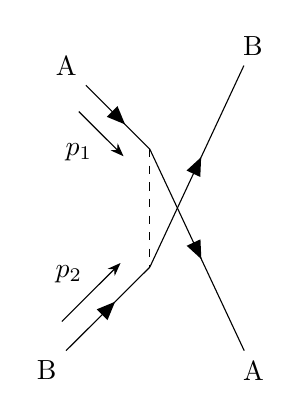
\begin{tikzpicture}
\begin{feynman}
\vertex (i1) {A};
\vertex [below right=of i1] (s1);
\vertex [below=of s1] (s2);
\vertex [below left=of s2] (i2) {B};
\vertex [above right=of s1] (f1) {B};
\vertex [below right=of s2] (f2) {A};
\diagram* {
(i1) -- [fermion, momentum'=\(p_1\)] (s1) -- [fermion] (f2),
(s1) -- [scalar] (s2),
(i2) -- [fermion, momentum=\(p_2\)] (s2) -- [fermion] (f1)
};
\end{feynman}
\end{tikzpicture}
\end{equation*}
To see this, consider the following computation,
\begin{align*}
\bra{0} \a_{p_2'}^B \a_{p_1'}^A \tfrac{i}{2} ( \bar{\psi}^{A'} \Gamma \psi^{A'}) (\bar{\psi}^{B'} \Gamma \psi^{B'})(\adag_{p_1})^A(\adag_{p_2})^B \ket{0} & = 
\contraction{\a_{p_2'}}{ \a_{p_1'}}{\tfrac{i}{2} ( }{\bar{\psi}}
\contraction[2ex]{}{ \a_{p_2'} }{ \a_{p_1'} \tfrac{i}{2} ( \bar{\psi} \Gamma \psi) (} {\bar{\psi}} 
\contraction{\a_{p_2'} \a_{p_1'} \tfrac{i}{2} ( \bar{\psi} \Gamma}{ \psi}{) (\bar{\psi} \Gamma \psi)}{\adag}
\contraction[2ex]{\a_{p_2'} \a_{p_1'} \tfrac{i}{2} ( \bar{\psi} \Gamma \psi) (\bar{\psi} \Gamma}{ \psi }{)\adag_{p_1}}{ \adag}
\a_{p_2'} \a_{p_1'} \tfrac{i}{2} ( \bar{\psi} \Gamma \psi) (\bar{\psi} \Gamma \psi)\adag_{p_1} \adag_{p_2} 
\\
& + 
\contraction{}{ \a_{p_2'}}{ \a_{p_1'}\tfrac{i}{2} ( }{\bar{\psi}}
\contraction[2ex]{\a_{p_2'} }{ \a_{p_1'} }{ \tfrac{i}{2} ( \bar{\psi} \Gamma \psi) (} {\bar{\psi}} 
\contraction{\a_{p_2'} \a_{p_1'} \tfrac{i}{2} ( \bar{\psi} \Gamma}{ \psi}{) (\bar{\psi} \Gamma \psi) \adag_{p_1}}{\adag}
\contraction[2ex]{\a_{p_2'} \a_{p_1'} \tfrac{i}{2} ( \bar{\psi} \Gamma \psi) (\bar{\psi} \Gamma}{ \psi }{)}{\adag}
\a_{p_2'} \a_{p_1'} \tfrac{i}{2} ( \bar{\psi} \Gamma \psi) (\bar{\psi} \Gamma \psi)\adag_{p_1} \adag_{p_2} 
\\
& = \tfrac{i}{2} ( \bar{u}_{p_1'} \Gamma u_{p_1}) (\bar{u}_{p_2'} \Gamma u_{p_2}) + \tfrac{i}{2} ( \bar{u}_{p_2'} \Gamma u_{p_2}) (\bar{u}_{p_1'} \Gamma u_{p_1}) 
\\
& = i ( \bar{u}_{p_1'} \Gamma u_{p_1}) (\bar{u}_{p_2'} \Gamma u_{p_2})
\end{align*}
where the other terms do not contribute since the $A$ and $B$ terms need to be contracted in the same factors when $A \neq B$. When $A = B$ then the four-point amplitude is identical to the one computed earlier, 
\[ i N \mathcal{M} = i ( \bar{u}_{p_1'} \Gamma u_{p_1}) (\bar{u}_{p_2'} \Gamma u_{p_2}) - i ( \bar{u}_{p_1'} \Gamma u_{p_2}) (\bar{u}_{p_2'} \Gamma u_{p_1}) \]
The rules for anti-particle scattering are similar in that only one of the two diagrams contributes when $A \neq B$ and when $A = B$ the tree-level amplitudes are identical to those computed using Wick's theorem earlier. 


\subsubsection{Leading Order Diagrams in the $N \to \infty$ Limit}

To make sensible predictions from this Lagrangian, we will need to perform renormalization. Therefore, we need some counterterms. I propose adding terms of the form,
\[ \lagrange_{\mathrm{ct}} = \bar{\psi}^A (c_Z i \slashed{\partial} - c_M) \psi^A + \frac{1}{2 N} ( \bar{\psi}^A \Gamma_{\mathrm{ct}} \psi^{A} ) ( \bar{\psi}^B \Gamma_{\mathrm{ct}} \psi^B) \]
where $\Gamma_{\mathrm{ct}} = g_e^{\mathrm{ct}} + g_0^{\mathrm{ct}} i \gamma^5$ is the counterterm interaction vertex which has the same overall form as the standard interaction vertex. 
\bigskip\\
For exactly the same reasons explained in problem set 5, to leading order in $N$ the only terms which contribute to $\psi^A \psi^B \to \psi^A \psi^B$ scattering for $A \neq B$ are ``bubble chains'' i.e. $t$-channel diagrams with a linear chain of loops in the interaction between the incoming particles. Diagrams with loops branching off these loops are exactly canceled by the mass and field strength renormalization which fixes the form of the exact propagator. The leading order terms under consideration look like,
\begin{figure}
\begin{center}
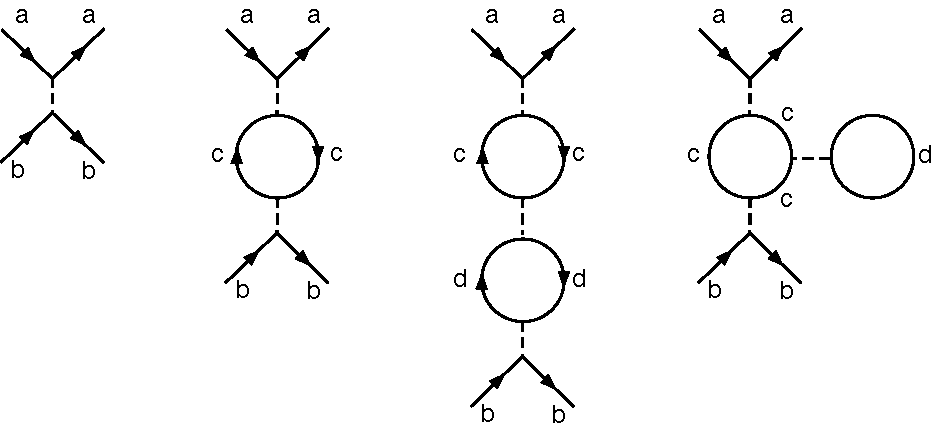
\includegraphics{leading-diagrams-UN}
\end{center}
\end{figure}
\noindent
Furthermore, any interaction line can be replaced with a counterterm line. Additionally, each $\phi$ propagator can be modified with a mass or field strength renormalization counterterm vertex. However, to leading order, the one-particle irreducible diagrams have branching ``loop trees'' like the diagram on the left rather than multiple connections to the propagator like the diagram on the right. 
\begin{figure}
\begin{center}
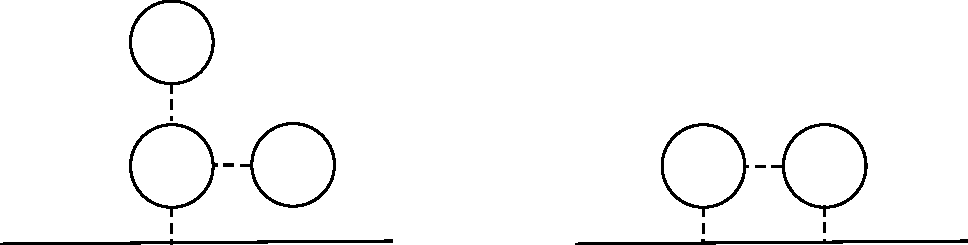
\includegraphics{UNtwopoint}
\end{center}
\end{figure}
\noindent
In such multiply connected diagrams, the total amount of momentum flowing into the loops depends both on the integration parameter and on the total incoming momentum. However, tree-like arrangements of loops have no cycles of momentum flow around the propagator so the total momentum flowing into the tree of loops is zero and thus constant. Therefore, these diagrams only give a (horribly UV divergent) constant shift to the particle mass and field strength. Using the renormalized physical parameters, the counterterm vertex must exactly cancel these ``loop trees'' and therefore, the addition of $\psi$ propagator counterterms in the ``bubble chain'' diagrams is exactly canceled by the chains with additional branching ``loop trees.'' There are also $u$ and $s$ channel diagrams such as,
\begin{equation}
\feynmandiagram [vertical = a to b, baseline = (a)] {
	a -- [anti fermion, edge label = A] t1 -- [anti fermion, edge label = A] i1,
	i2 -- [anti fermion, edge label = A] t2 -- [anti fermion, edge label = A] a, 
	t1 -- [scalar] t2,
	a -- [scalar] b,
	o1 -- [fermion, edge label = B] b -- [fermion, edge label = B] o2
};
\end{equation}
However, the $\phi$ fields which contribute to the loops in such diagrams are constrained to be of type $A$ (or type $B$ for the flipped diagram) and therefore the loop does not contribute an extra summation over particle types. Therefore, these diagrams are suppressed by a factor of $1/N$ so we will not include them in our $N \to \infty$ limit.  

\subsection{Trace Tricks}

We're going to need some serious trace machinery specialized for $D = 1 + 1$ dimensions to simplify the scattering cross sections. Fist, note that $\gamma^5 = \gamma^0 \gamma^1$. Therefore, $\{ \gamma^5, \gamma^\mu \} = 0$ and $(\gamma^5)^2 = \mathrm{1}$.

\begin{proposition}
I will make use of these trace tricks,
\begin{enumerate}
\item[1.] $\tr{\gamma^\mu } = \tr{\gamma^5} = 0$.

\item[2.] The trace of any odd number of gamma matrices is zero.

\item[3.] The trace of $\gamma^5$ times an odd number of gamma matrices is zero.

\item[4.] $ \tr{ \gamma^\mu \gamma^\nu} = 2 \eta^{\mu \nu} $

\item[5.] $ \tr{ \gamma^\mu \gamma^\nu \gamma^5 } =  2 \epsilon^{\mu \nu}$
\end{enumerate}
\end{proposition}

\begin{proof}
The first can be checked by a direct computation. The second and third properties follow directly from the (anti)commutation relations\footnote{Peskin and Schoeder Chapter 5.1, Trace Technology, page 133.}.
Consider,
\[ \tr{\gamma^\mu \gamma^\nu} = \tr{\gamma^\nu \gamma^\mu} = \tfrac{1}{2} \tr{ \{ \gamma^\mu, \gamma^\nu \} } = \tr{\eta^\mu \nu} = 2 \eta^{\mu \nu} \]
Furthermore,
\[ \tr{\gamma^\mu \gamma^\nu \gamma^5} = -\tr{\gamma^\nu \gamma^\mu \gamma^5} + 2 \eta^{\mu \nu} \tr{\gamma^5} = - \tr{\gamma^\nu \gamma^\mu \gamma^5} \]
Therefore, $\tr{\gamma^\mu \gamma^\nu \gamma^5}  \propto \epsilon^{\mu \nu}$. Evaluating a special case will give the desired coefficient,
\[ \tr{\gamma^0 \gamma^1 \gamma^5} = \tr{\gamma^0 \gamma^1 \gamma^0 \gamma^1} = - \tr{(\gamma^5)^2} = 2\]
\end{proof}
\noindent
I will use these properties to derive some important properties of traces of combinations of $\slashed{p}$ and $\Gamma$. 

\begin{proposition}

\item[1] $ \tr{ \Gamma } = 2 \gs $ and $\tr{ \Gamma^2 } = 2 \left( \gs^2 - \gp^2 \right)$ 

\item[2] $ \tr{ \slashed{p} \Gamma } = \tr{ \slashed{p} } = \tr{ \Gamma \slashed{p} \Gamma } = 0 $ 

\item[3] $  \tr{ \slashed{p} \Gamma \slashed{q} \Gamma } = (\gs^2 + \gp^2) \tr{ \slashed{p} \slashed{q} } = 4 (\gs^2 + \gp^2) p \cdot q $

\item[4] $\tr{ (\slashed{p} + \eta_p m) \Gamma (\slashed{q} + \eta_q m) \Gamma } = 2 ( \gs^2 + \gp^2) p \cdot q + 2 \eta_p \eta_q m^2 (\gs^2 - \gp^2) $

\item[5] $\tr{ (\slashed{p} \pm m) \Gamma (\slashed{q} \pm m) \Gamma } = 2 ( \gs^2 + \gp^2) p \cdot q + 2 m^2 (\gs^2 - \gp^2)$ 
\end{proposition}

\begin{proof}

First, $\tr{ \Gamma } = \tr{ \gs + i \gp \gamma^5 } = \tr { \gs } = 2 \gs$ and
 \[\tr{ \Gamma^2 } = \tr{ \gs^2 - \gp^2 + 2 i \gs \gp \gamma^5 } =  2 \left( \gs^2 - \gp^2 \right)\] 
\bigskip\\
$ \tr{ \slashed{p} } = \tr{ \gamma^\mu p_\mu } = p_\mu \tr{ \gamma^\mu} = 0 $ and $ \tr{ \slashed{p} \Gamma } = p_\mu \tr{ \gamma^\mu (\gs + i \gp \gamma^5 ) } = 0$ and 
\[ \tr{ \Gamma \slashed{p} \Gamma } = p_\mu \tr{ \gamma^\mu \Gamma^2} = p_\mu \tr{ \gamma^\mu (\gs^2 - \gp^2 + 2 i \gs \gp \gamma^5) } = 0 \]
\bigskip\\
\begin{align*} 
\tr{ \slashed{p} \Gamma \slashed{q} \Gamma } & = p_\mu q_\nu \tr{ \gamma^\mu (\gs + i \gp \gamma^5 ) \gamma^\nu ( \gs + i \gp \gamma^5 ) }  = \tr{ \gamma^\mu \gamma^\nu ( \gs - i \gp \gamma^5) (\gs + i \gp \gamma^5) } 
\\
& = p_{\mu} q_{\nu} \tr{ \gamma^\mu \gamma^\nu (\gs^2 + \gp^2) } = p_\mu q_\nu 4 (\gs^2 + \gp^2)\eta^{\mu \nu} = 2 (\gs^2 + \gp^2)  p \cdot q 
\end{align*}
\bigskip\\
\begin{align*}
\tr{ (\slashed{p} + \eta_p m) \Gamma (\slashed{q} + \eta_q m) \Gamma } & = \tr{ \slashed{p} \Gamma \slashed{q} \Gamma } + \tr{ \eta_p m \Gamma \slashed{q} \Gamma } + \tr{ \slashed{p} \Gamma \eta_q m \Gamma } + \tr{ \eta_p \eta_q m^2 \Gamma^2 } 
\\
& = 2 ( \gs^2 + \gp^2) p \cdot q + 2 \eta_p \eta_q m^2 (\gs^2 - \gp^2) 
\end{align*}
since the middle terms are zero. Now I will define some quantities to simplify the calculations, the total coupling $g^2 = g_e^2 + g_o^2$ and the coupling shift $\delta = g_e^2 - g_o^2$.  
\end{proof}

\subsubsection{Calculating the Loop Integral}
Consider the loop component,
\begin{equation}
\feynmandiagram [vertical' = d to b, inline=(l1.base), tree layout] {
b -- [scalar] l1 
-- [fermion, half left, looseness=1.5, momentum = \(k\)] l2 
--[fermion, half left, looseness=1.5, momentum =\(p + k\)] l1,
l2 -- [scalar] d
}; 
= - \frac{i^2N}{N^2} \frac{\tr{ \Gamma ((\slashed{p} + \slashed{k}) + m) \Gamma (\slashed{k} + m) } }{((p+k)^2 - m^2 + i \epsilon)(k^2 - m^2 + i \epsilon)} 
\end{equation}
Using our trace tricks and introducing Feynman parameters,
\begin{align*}
i V(p) & =  \int \frac{\dn{2}{k}}{(2\pi)^2} \frac{\tr{ \Gamma ((\slashed{p} + \slashed{k}) + m) \Gamma (\slashed{k} + m) } }{((p+k)^2 - m^2 + i \epsilon)(k^2 - m^2 + i \epsilon)} 
\\
& = \int \frac{\dn{2}{k}}{(2\pi)^2} \int_0^1 \d{x} \d{y} \frac{ 2 g^2 (k^2 + p \cdot k) + 2 m^2 \delta }{( x (p + k)^2  + y k^2 - m^2 + i \epsilon  )^2} \delta(x + y - 1)
\\
& = \int \frac{\dn{2}{k}}{(2\pi)^2} \int_0^1 \d{x} \d{y} \frac{ 2 g^2 (k^2 + p \cdot k) + 2 m^2 \delta }{( k^2 + 2 x p \cdot k + x p^2 - m^2 + i \epsilon  )^2} \delta(x + y - 1)
\\
& = \int \frac{\dn{2}{k}}{(2\pi)^2} \int_0^1 \d{x} \d{y} \frac{ 2 g^2 (k^2 + p \cdot k) + 2 m^2 \delta }{( (k + x p)^2 + (x - x^2) p^2 - m^2 + i \epsilon  )^2} \delta(x + y - 1)
\\
& = \int \frac{\dn{2}{\ell}}{(2\pi)^2} \int_0^1 \d{x} \d{y} \frac{ 2 g^2 ((\ell -xp)^2 + p \cdot (\ell - xp)) + 2 m^2 \delta }{( \ell^2 + (x - x^2) p^2 - m^2 + i \epsilon  )^2} \delta(x + y - 1)
\\
& = \int \frac{\dn{2}{\ell}}{(2\pi)^2} \int_0^1 \d{x} \d{y} \frac{ 2 g^2 \ell^2 + 2 g^2 (x^2 - x) p^2 + 2 m^2 \delta}{( \ell^2 + (x - x^2) p^2 - m^2 + i \epsilon  )^2} \delta(x + y - 1)
\end{align*}
using the fact that terms linear in $\ell$ are odd and thus integrate to zero. Now define the constant,
\[\Delta = (x^2 - x) p^2 + m^2 - i \epsilon \] 
perform a Wick rotation, and introduce a Schwinger parameter,
\begin{align*}
i V(p) & = -i \int \frac{\dn{2}{\ell_E}}{(2\pi)^2} \int_0^1 \d{x} \d{y} \frac{ 2 g^2 \ell_E^2 - 2 g^2 (x^2 - x) p^2 - 2 m^2 \delta}{( \ell_E^2 + \Delta  )^2} \delta(x + y - 1)
\\
& = -i \int \frac{\dn{2}{\ell_E}}{(2\pi)^2} \int_0^1 \d{x} \d{y} [ 2 g^2 \ell_E^2 - 2 g^2 (x^2 - x) p^2 - 2 m^2 \delta] \: \delta(x + y - 1) \int_0^\infty \frac{\d{s}}{s} s^2 e^{-s (\ell_E^2 + \Delta)} 
\end{align*} 
To evaluate this integral, we perform dimensional regularization by integrating in $D  = 2 - \delta_D$ dimensions. Thus, 
\begin{align*}
i V(p) & = -i \int \frac{\dn{D}{\ell_E}}{(2\pi)^D} \int_0^1 \d{x} \d{y} [ 2 g^2 \ell_E^2 - 2 g^2 (x^2 - x) p^2 - 2 m^2 \delta] \: \delta(x + y - 1) \int_0^\infty \frac{\d{s}}{s} s^2 e^{-s (\ell_E^2 + \Delta)} 
\\
& = -2 i \int_0^1 \d{x} \int_0^\infty \frac{\d{s}}{s} s^2 \int_0^\infty \frac{\d{\ell_E} \, \ell_E^{D-1}}{(4\pi)^{D/2} \Gamma\left(\frac{D}{2}\right)} [ 2 g^2 \ell_E^2 - 2 g^2 (x^2 - x) p^2 - 2 m^2 \delta] e^{-s(\ell_E^2 + \Delta)} 
\\
& = -2 i \int_0^1 \d{x} \int_0^\infty \frac{\d{s}}{s} s^2 e^{-s \Delta} \int_0^\infty \frac{\d{\ell_E} \, \ell_E^{D-1}}{(4\pi)^{D/2} \Gamma\left(\frac{D}{2}\right)} [ 2 g^2 \ell_E^2 - 2 g^2 (x^2 - x) p^2 - 2 m^2 \delta] e^{-s \ell_E^2} 
\end{align*} 
By a change of variables $u = s \ell_E$ we can write the integral,
\[ \int_0^\infty \d{\ell_E} \: \ell_E^{D - 1} e^{-s \ell_E^2}  = \frac{1}{2 s} \frac{1}{s^{\frac{D}{2} - 1}} \int_0^\infty \d{u} u^{\frac{D}{2} - 1} e^{-u} = \frac{\Gamma\left(\tfrac{D}{2}\right)}{2 s^{\frac{D}{2}}}  \]
Therefore,
\begin{align*}
i V(p) 
& = -\frac{i}{(4 \pi)^{D/2}} \int_0^1 \d{x} \int_0^\infty \frac{\d{s}}{s} s^{2 - \frac{D}{2}} e^{-s \Delta} \left[ 2 g^2 \frac{D}{2s} - 2 g^2 (x^2 - x) p^2 - 2 m^2 \delta \right]
\\
& = -\frac{i}{(4 \pi)^{D/2}} \int_0^1 \d{x} \int_0^\infty \frac{\d{s}}{s} s^{2 - \frac{D}{2}} e^{-s \Delta} \left[ 2 g^2 \frac{D}{2s} - 2 g^2 (x^2 - x) p^2 - 2 m^2 \delta \right]
\\
& = -\frac{i}{(4 \pi)^{D/2}} \int_0^1 \d{x} \left[ \left(2 g^2  \frac{D}{2} \right) \frac{\Gamma \left(1 - \frac{D}{2} \right)}{\Delta^{1 - \frac{D}{2}}} - \left( 2 g^2 (x^2 - x) p^2 + 2 m^2 \delta \right) \frac{\Gamma \left(2 - \frac{D}{2} \right)}{\Delta^{2 - \frac{D}{2}}} \right]
\end{align*} 
For $D = 2 - \delta_D$ we have $\Gamma\left(2 - \frac{D}{2}\right) = \Gamma(1 + \tfrac{1}{2} \delta_D) \xrightarrow{\delta_D \to 0} 1$ and $\Gamma\left(1 - \frac{D}{2}\right) = \Gamma(\tfrac{1}{2} \delta_D) \xrightarrow{\delta_D \to 0} \frac{2}{\delta_D} - \gamma + O(\delta_D)$.
Using the fact that,
\[ \lim\limits_{\delta \to 0} \frac{1 - Q^{-\delta/2}}{\delta/2} =  \lim\limits_{\delta \to 0} \int_1^Q x^{-\delta/2 - 1} \: \d{x} = \int_1^Q \lim\limits_{\delta \to 0^-} x^{-\delta/2 - 1} \: \d{x}  = \int_1^Q \lim\limits_{\delta \to 0} x^{- 1} \: \d{x} = \log{Q} \]
and plugging in,
\begin{align*}
i V(p) 
& = -\frac{i}{4 \pi} \int_0^1 \d{x} \left[ \left(2 g^2  \frac{2 - \delta_D}{2} \right) \frac{\frac{2}{\delta_D} - \gamma + O(\delta_D) }{[(4\pi)^{-1} \Delta]^{\frac{1}{2} \delta_D}} - \left( 2 g^2 (x^2 - x) p^2 + 2 m^2 \delta \right) \frac{1}{\Delta} \right]
\\
& \xrightarrow{\delta_D \to 0}  -\frac{i}{4 \pi} \int_0^1 \d{x}
\\
& \quad \quad \quad \cdot \left[ 2 g^2 \left( \frac{2}{\delta_D} - \log{\left[(4 \pi)^{-1} \Delta \right]} - \gamma + O(\delta_D) - 1 \right) - \frac{ 2 g^2 (x^2 - x) p^2 + 2 m^2 \delta }{\Delta} \right]
\\
& = \frac{i}{4 \pi} \int_0^1 \d{x}
\\
& \quad \quad \cdot \left[ 2 g^2 \left(\log{[ x(x-1) p^2 + m^2 - i \epsilon]} - \log{(4 \pi)} - \frac{2}{\delta_D} + \gamma + 1 + O(\delta_D) \right) + \frac{ 2 g^2 x(x - 1) p^2 + 2 m^2 \delta }{x(x-1) p^2 + m^2 - i \epsilon} \right]
\end{align*} 

\subsubsection{The Large $N$ Limit Scattering Amplitude}

Since the divergent terms in the loop integral do not have any momentum dependence, we can take the form of the vertex counterterm to simply be $\Gamma_{\mathrm{ct}} = \sqrt{c_g} \Gamma$. In this case, the simple four-point interaction vertex with $A \neq B$ is modified to give the amplitude,
\[ i ( \bar{u}_{p_1'} \Gamma u_{p_1}) (\bar{u}_{p_2'} \Gamma u_{p_2}) + c_g i ( \bar{u}_{p_1'} \Gamma u_{p_1}) (\bar{u}_{p_2'} \Gamma u_{p_2}) = ( \bar{u}_{p_1'} \Gamma u_{p_1}) i(1 + c_g) (\bar{u}_{p_2'} \Gamma u_{p_2}) \]
Since changing any vertex into a counterterm vertex gives another valid diagram in the sum, we may simplify the calculation by incorporating these two types of vertices into a single vertex with coefficient $i(1 + c_g)$. Then, the sum over bubble chains gives an amplitude,
\[ i \mathcal{M} = ( \bar{u}_{p_1'} \Gamma u_{p_1}) \left[ \frac{i(1 + c_g)}{N} + N \left( \frac{i(1 + c_g)}{N} \right)^2 i V(t) + N^2 \left( \frac{i(1 + c_g)}{N} \right)^3 [i V(p)]^2 + \cdots  \right] (\bar{u}_{p_2'} \Gamma u_{p_2}) \]
where $i V(p)$ is the amplitude of the single loop diagram with total incoming momentum $p$. This formula holds because there is always one more interaction vertex than the number of loops in the chain and the outgoing momentum of each loop is equal to its incoming momentum so each loop has a total of $p$ momentum flowing through it. In the case of $\psi^A \psi^B \to \psi^A \psi^B$ scattering the diagrams occur in the $t$-channel so $p^2 =  t$. We can simplify this amplitude by noting that the sum is a geometric series,

\begin{align*}
i \mathcal{M} & = (\bar{u}_{p_1'} \Gamma u_{p_1}) \frac{i(1 + c_g)}{N} \left[ 1 - (g + c_g) V(p) + [(g + c_g) V(p)]^2 + \cdots \right] (\bar{u}_{p_2'} \Gamma u_{p_2}) 
\\
& = (\bar{u}_{p_1'} \Gamma u_{p_1}) \frac{i(1 + c_g)}{N} \cdot \frac{1}{1 + (1 + c_g) V(p)} (\bar{u}_{p_2'} \Gamma u_{p_2}) 
\end{align*}


\subsubsection{Renormalization}

We choose to renormalize at zero momentum. Therefore, we will take the renormalization point $t = 0$. At the renormalization point, we require that the coupling vertex at tree-level $\Gamma$ equals the physical interaction. That is,
\[ i \mathcal{M}(t = 0) = (\bar{u}_{p_1'} \Gamma u_{p_1}) \frac{i(1 + c_g)}{N} \cdot \frac{1}{1 + (1 + c_g) V(t = 0)} (\bar{u}_{p_2'} \Gamma u_{p_2}) = (\bar{u}_{p_1'} \Gamma u_{p_1}) \frac{i}{N} (\bar{u}_{p_2'} \Gamma u_{p_2}) \]
Therefore, we need to set,
\[ \frac{1 + c_g}{1 + (1 + c_g) Q} = 1 \]
where I have defined,
\[ Q = V(t = 0) = \frac{1}{4 \pi} \int_0^1 \d{x} \left[ 2 g^2 \left(\log{ m^2 } - \log{(4 \pi)} - \frac{2}{\delta_D} + \gamma + 1 + O(\delta_D) \right) + \frac{ 2 m^2 \delta }{ m^2 } \right] \]
and I have taken the limit $\epsilon \to 0$ since the integral has no branch cuts since $m > 0$. The renormalization condition set,
\[ 1 + c_g = 1 + (1 + c_g) Q \implies c_g(1 - Q) = Q \implies c_g = \frac{Q}{1 - Q} \]
Therefore,
\[ 1 + c_g = \frac{1}{1 - Q} \]
which when replaced in the general form of the scattering amplitude gives the renormalized expression,
\[ i \mathcal{M} = (\bar{u}_{p_1'} \Gamma u_{p_1}) \frac{\frac{i}{1 - Q}}{N} \cdot \frac{1}{1 + \frac{1}{1 - Q} V(t)} (\bar{u}_{p_2'} \Gamma u_{p_2}) = (\bar{u}_{p_1'} \Gamma u_{p_1}) \frac{i}{N} \cdot \frac{1}{1 + V(t) - Q} (\bar{u}_{p_2'} \Gamma u_{p_2}) 
\]
Therefore, consider the term,
\begin{align*}
V(t) - Q & = \frac{1}{4 \pi} \int_0^1 \d{x} \left[ 2 g^2 \log \left[ \frac{x(1 - x) |t| + m^2}{m^2} \right] + \frac{2g^2 x(1-x) |t| + 2 m^2 \delta}{x(1-x) |t| + m^2} - 2 \delta \right]
\end{align*}
I have taken the limit $\epsilon \to 0$ because $t < 0$ in the normal two-particle scattering regime so the arguments are all strictly positive so we do not need to worry about branch cuts. Furthermore, in the center of mass frame for nontrivial scattering we can write,
In the center of mass frame we write,
\[ p_1 = (E, p) \quad p_2 = (E, -p) \quad p_1' = (E, -p) \quad p_2' = (E, p) \]
In these variables, the spinor factors evaluate to,
\[  (\bar{u}_{p_1'} \Gamma u_{p_1})(\bar{u}_{p_2'} \Gamma u_{p_2}) = 4 \left( g_e^2 m^2 + g^2 p^2 \right) \]
Finally, putting everything together,
\[ i \mathcal{M} = \frac{i}{N} \cdot \frac{4 \left( g_e^2 m^2 + g^2 p^2 \right)}{1 + V(t) - Q} \]


\subsubsection{High Energy Behavior}

Consider the limit $|t| \gg m^2$. Then we can approximate,
\begin{align*}
V(t) - Q & = \frac{1}{4 \pi} \int_0^1 \d{x} \left[ 2 g^2 \log \left[ \frac{x(1 - x) |t| + m^2}{m^2} \right] + \frac{2g^2 x(1-x) |t| + 2 m^2 \delta}{x(1-x) |t| + m^2} - 2 \delta \right]
\\
& \approx \frac{1}{4 \pi} \int_0^1 \d{x} \left[ 2 g^2 \log \left[ \frac{x(1 - x) |t|}{m^2} \right] + \frac{2g^2 x(1-x) |t| }{x(1-x) |t|} - 2 \delta \right]
\\
& = \frac{1}{4 \pi} \int_0^1 \d{x} \left[ 2 g^2 \log{x(1 - x)} + 2g^2 \log{ \frac{|t|}{m^2} } + 2 g^2 - 2 \delta \right]
\\
& = \frac{1}{2 \pi} \left[ g^2 \log{ \frac{|t|}{m^2} } - g^2 - \delta \right] 
\end{align*}
therefore,
\[ i \mathcal{M} = \frac{i}{N} \cdot \frac{ 4 \left( g_e^2 m^2 + g^2 p^2 \right) }{1 + \frac{1}{2 \pi} \left[ g^2 \log{ \frac{|t|}{m^2} } - 2 g_e^2 \right] } \]
Using our formula for the scattering cross section we get,
\[ \sigma = \frac{\left( g_e^2 m^2 + g^2 p^2 \right)^2}{N^2 p^2 \Ecm^2} \cdot \frac{1}{\left( 1 + \frac{1}{2 \pi} \left[ g^2 \log{ \frac{|t|}{m^2} } - 2 g_e^2 \right] \right)^2} \]
As $|t| \to \infty$ the scattering cross section $\sigma \to 0$. Therefore, this theory exhibits asymptotic freedom in the large $N$ limit. This is the opposite behavior from the bosonic quartic theory considered in problem set 5 which exhibited a pole in the effective coupling constant at high energy. At high energy in this theory, the theory becomes effectively free rather than infinitely strongly coupled as did the bosonic theory. 

\subsubsection{An Alternative Renormalization Scheme}

Now, we choose to renormalize at the point $N \mathcal{M}(t = -\mu^2) = ( \bar{u}_{p_1'} \Gamma u_{p_1}) (\bar{u}_{p_2'} \Gamma u_{p_2})$ such that tree-level is exact at $t = - \mu^2$. Consider a scale-dependent effective coupling constants $g_e(\mu)$ and $g_o(\mu)$ which are solutions to the previous renormalization condition. Then, exactly as before, we get,
\[ 
\frac{1 + c_g}{1 + (1 + c_g) V(-\mu^2)} = 1 \implies c_g  = \frac{V(-\mu^2)}{1 - V(-\mu^2)} \implies 1 + c_g = \frac{1}{1 - V(-\mu^2)} 
\]
Therefore, 
\[ 
i \mathcal{M}(t) = \frac{i}{N} \cdot \frac{4 \left( g_e^2(\mu) m^2 + g^2(\mu) p^2 \right)}{1 + V(t) - V(-\mu^2)} 
\]
Now, in the limit $\mu^2 \gg m^2$ and $|t| \gg m^2$ we can easily evaluate the denominator. Consider,
\begin{align*}
V(t) - V(-\mu^2) & = \frac{1}{4 \pi} \int_0^1 \d{x} \left[ 2 g^2 \log \left[ \frac{x(1 - x) |t| + m^2}{x(1-x) \mu^2 + m^2} \right] + \frac{2g^2 x(1-x) |t| + 2 m^2 \delta}{x(1-x) |t| + m^2} - \frac{2 g^2 x(1 - x) \mu^2 + 2 m^2 \delta}{x (1 - x) \mu^2 + m^2} \right]
\\
& \approx \frac{1}{4 \pi} \int_0^1 \d{x} \left[ 2 g^2 \log \left[ \frac{x(1 - x) |t|}{x(1 - x)m^2} \right] + \frac{2g^2 x(1-x) |t| }{x(1-x) |t|} - \frac{2g^2 x(1-x) \mu^2 }{x(1-x) \mu^2} \right]
\\
& = \frac{1}{4 \pi} \int_0^1 \d{x} \left[ 2g^2 \log{ \frac{|t|}{\mu^2} }  \right]
\\
& = \frac{g^2}{2 \pi} \log{\frac{|t|}{\mu^2}}
\end{align*}
Plugging into the expression for the scattering amplitude,
\[ i \mathcal{M}(t) = \frac{i}{N} \cdot \frac{4 \left( g_e^2(\mu) m^2 + g^2(\mu) p^2 \right)}{1 + \frac{1}{2\pi} {[g_e^2(\mu) + g_o^2(\mu)]} \log{ \frac{|t|}{\mu^2} }} \]
This expression is well-defined in the limit $m \to 0$ and $t \to 0$ since the denominator diverges and the numerator goes to zero. Therefore, in the limit $m \to 0$ and $t \to 0$ we have $\mathcal{M} \to 0$. Therefore, massless particles become decoupled in this theory both at high and low energy.  
\bigskip\\
However, the above discusses renormalization at a single point which does not seem to give enough information to solve for two coupling constants. Therefore, we should consider this discussion somewhat more carefully. First we start off as generally as possible. Let $\Gamma(\mu)$ be the scale-dependent (matrix) vertex coupling. If we renormalize at the point $t = -\mu^2$ then we require that the tree-level scattering amplitude using the scale-dependent vertex is equal to the exact result at $t = -\mu^2$. That is,
\[ N \mathcal{M}(t = -\mu^2) = ( \bar{u}_{p_1'} \Gamma(\mu) u_{p_1}) (\bar{u}_{p_2'} \Gamma(\mu) u_{p_2}) = ( \bar{u}_{p_1'} \Gamma u_{p_1}) \frac{1}{1 + V(-\mu^2) - Q} (\bar{u}_{p_2'} \Gamma u_{p_2}) \]
However, both sides will have the same matrix form if we take,
\[ \Gamma(\mu) = \Gamma \alpha(\mu) \]
and thus $g_e(\mu) = \alpha(\mu) g_e$ and $g_o(\mu) = \alpha(\mu) e_o$ for some proportionality constant $\alpha$. 
Therefore, in the limit $|t| \gg m^2$ we have,
\[ \alpha^2(\mu) = \frac{1}{1 + V(-\mu^2) - Q} = \frac{1}{1 + \frac{1}{2\pi} \left[ g^2 \log{\frac{|t|}{m^2}} - 2 g_e^2 \right]} \]
Therefore,
\begin{align*}
N \mathcal{M}(t) & = ( \bar{u}_{p_1'} \Gamma(\mu) u_{p_1}) \frac{\alpha^{-2}(\mu)}{1 + V(t) - Q} (\bar{u}_{p_2'} \Gamma(\mu) u_{p_2}) 
\\
& = ( \bar{u}_{p_1'} \Gamma(\mu) u_{p_1}) \frac{\alpha^{-2}(\mu)}{1 + V(t) - V(-\mu^2) + V(-\mu^2) - Q} (\bar{u}_{p_2'} \Gamma(\mu) u_{p_2})
\\
& = ( \bar{u}_{p_1'} \Gamma(\mu) u_{p_1}) \frac{\alpha^{-2}(\mu)}{\alpha^{-2}(\mu) + V(t) - V(-\mu^2)} (\bar{u}_{p_2'} \Gamma(\mu) u_{p_2})
\\
& = ( \bar{u}_{p_1'} \Gamma(\mu) u_{p_1}) \frac{1}{1 + \alpha^2(\mu)[ V(t) - V(-\mu^2)]} (\bar{u}_{p_2'} \Gamma(\mu) u_{p_2})   
\end{align*}
In the limit $|t| \gg m^2$ we have calculated the integral,
\[ V(t) - V(-\mu^2) = \frac{g^2}{2 \pi} \log{\frac{|t|}{\mu^2}} \]
Therefore, we have,
\[ N \mathcal{M}(t) = ( \bar{u}_{p_1'} \Gamma(\mu) u_{p_1}) \frac{1}{1 + \frac{1}{2\pi} g^2 \alpha^2(\mu) \log{\frac{|t|}{\mu^2}} } (\bar{u}_{p_2'} \Gamma(\mu) u_{p_2}) = ( \bar{u}_{p_1'} \Gamma(\mu) u_{p_1}) \frac{1}{1 + \frac{1}{2\pi} g^2(\mu) \log{\frac{|t|}{\mu^2}} } (\bar{u}_{p_2'} \Gamma(\mu) u_{p_2}) \]
which is the same expression we derived earlier. 


\subsubsection{The Beta Function}

The running of coupling constants can be derived from looking at leading order Feynman diagrams. We choose the renormalization condition that the tree-level scattering amplitude using the scale-dependent vertex is equal to the exact result at the point $t = -\mu^2$. That is,
\[ N \mathcal{M}(t = -\mu^2) = ( \bar{u}_{p_1'} \Gamma(\mu) u_{p_1}) (\bar{u}_{p_2'} \Gamma(\mu) u_{p_2}) = ( \bar{u}_{p_1'} \Gamma u_{p_1}) \frac{1}{1 + V(-\mu^2) - Q} (\bar{u}_{p_2'} \Gamma u_{p_2}) \] 
Then, consider the amplitude, 
\[ ( \bar{u}_{p_1'} \Gamma(e^\varepsilon \mu) u_{p_1}) (\bar{u}_{p_2'} \Gamma(e^\varepsilon \mu) u_{p_2}) = N \mathcal{M}(t = -(e^\varepsilon \mu)^2) \]
Consider the Feynman diagram expansion to leading order in $\frac{1}{N}$, 
which give amplitudes,
\[ i\mathcal{M} =  ( \bar{u}_{p_1'} \Gamma(\mu^2) u_{p_1}) \left[  \frac{i}{N} + \frac{i c_g}{N} + N \left(\frac{i}{N}\right)^2 iV(t) + \cdots \right] (\bar{u}_{p_2'} \Gamma(\mu^2) u_{p_2}) \] 
Using our renormalization condition,
\[ \frac{i}{N} = \frac{i}{N} + \frac{ic_g}{N} - \frac{i}{N} V(-\mu^2) + \cdots \]
and therefore,
\[ i\mathcal{M} =  ( \bar{u}_{p_1'} \Gamma u_{p_1}) \left[  \frac{i}{N} - \frac{i}{N} [V(t) - V(-\mu^2)] + \cdots \right] (\bar{u}_{p_2'} \Gamma u_{p_2}) \] 
In particular,
\[ \alpha^2(e^\varepsilon \mu) = \alpha^2(\mu) \left[ 1 - [V(t) - V(-\mu^2)] + \cdots \right] \] 
where the higher terms depend on larger powers in $V(-(e^\varepsilon \mu)^2) - V(-\mu^2)$. 
Now, in the high energy limit $\mu^2 \gg M^2$, we can evaluate the integral,
\begin{align*}
V(-&(e^\varepsilon \mu)^2) - V(-\mu^2)
\\
& = \frac{1}{4 \pi} \int_0^1 \d{x} \left[ 2 g^2 \log \left[ \frac{x(1 - x) e^{2\epsilon} \mu^2 + m^2}{x(1-x) \mu^2 + m^2} \right] + \frac{2g^2 x(1-x) e^{2\epsilon} \mu^2 + 2 m^2 \delta}{x(1-x) e^{2 \epsilon} + m^2} - \frac{2 g^2 x(1 - x) \mu^2 + 2 m^2 \delta}{x (1 - x) \mu^2 + m^2} \right]
\\
& \approx \frac{1}{4 \pi} \int_0^1 \d{x} \left[ 2 g^2 \log \left[ \frac{x(1 - x) e^{2\epsilon} \mu^2}{x(1 - x)m^2} \right] + \frac{2g^2 x(1-x) e^{2\epsilon} \mu^2 }{x(1-x) e^{2\epsilon} \mu^2} - \frac{2g^2 x(1-x) \mu^2 }{x(1 - x) \mu^2} \right]
\\
& = \frac{1}{4 \pi} \int_0^1 \d{x} \left[ 2g^2 \log{ \frac{e^{2\epsilon} \mu^2}{\mu^2} }  \right]
\\
& = g^2(\mu) \frac{\epsilon}{\pi}
\end{align*}
Therefore, because $V(-(e^\varepsilon \mu)^2) - V(-\mu^2)$ is order $\epsilon$ and the latter terms contain higher powers of this quantity,
\[ \alpha^2(e^\varepsilon \mu) = \alpha^2(\mu) - \alpha^4(\mu) (g_e^2 + g_o^2) \frac{\epsilon}{\pi} + O(\epsilon^2) \] 
Therefore,
\[ \deriv{\alpha}{\log{\mu}} = -\frac{g^2 \alpha^3(\mu)}{2 \pi} = \beta(\alpha(\mu)) \quad \text{where} \quad \beta(\alpha) = -\frac{g^2 \alpha^3}{2 \pi} \]
Immediately, we find that this theory exhibits asymptotic freedom because the beta function is negative. Therefore, the effective coupling decreases as the energy scale increases. Integrating this differential equation,
\[ \int_{\alpha_0}^{\alpha(\mu)} \frac{\d{\alpha}}{\alpha^3} = -\frac{g^2}{2 \pi}\int_{\log{\mu_0}}^{\log{\mu}} \d{\log{\mu}} \implies \frac{1}{2} \left[ \frac{1}{\alpha_0^2} - \frac{1}{\alpha^2(\mu)} \right] = -\frac{1}{2 \pi} \log{\frac{\mu}{\mu_0}} \]
which becomes,
\[ \alpha^2(\mu) = \frac{\alpha_0^2}{1 + \frac{\alpha_0^2 g^2}{\pi} \log{\frac{\mu}{\mu_0}}} \]
Since by definition $\Gamma(\mu) = \Gamma \alpha(\mu)$ we have also found the scattering amplitude at any energy scale. Setting, $\mu = \sqrt{|t|}$ we get,
\begin{align*} N \mathcal{M}(t) 
& = ( \bar{u}_{p_1'} \Gamma(|t|^{1/2}) u_{p_1}) (\bar{u}_{p_2'} \Gamma(|t|^{1/2}) u_{p_2})
\\
& = ( \bar{u}_{p_1'} \Gamma u_{p_1}) \alpha^2(|t|^{1/2}) (\bar{u}_{p_2'} \Gamma u_{p_2}) 
\\
& = ( \bar{u}_{p_1'} \Gamma u_{p_1}) \frac{\alpha_0^2}{1 + \frac{\alpha_0^2 g^2}{\pi} \log{\frac{|t|^{1/2}}{\mu_0}}} (\bar{u}_{p_2'} \Gamma u_{p_2}) 
\end{align*}
Using the fact that $\Gamma \alpha_0 = \Gamma(\mu_0)$ we can rewrite this expression as,
\[ i \mathcal{M}(t) = \frac{i}{N} \cdot ( \bar{u}_{p_1'} \Gamma(\mu_0) u_{p_1}) \frac{1}{1 + \frac{1}{2 \pi} g^2(\mu_0^2) \log{\frac{|t|}{\mu_0^2}}} (\bar{u}_{p_2'} \Gamma(\mu_0) u_{p_2}) \]
This is an identical expression for the scattering amplitude derived in the previous section renormalized at the point $\mu_0$.



\end{document}